\documentclass[11pt]{article}

    \usepackage[breakable]{tcolorbox}
    \usepackage{parskip} % Stop auto-indenting (to mimic markdown behaviour)
    
    \usepackage{iftex}
    \ifPDFTeX
    	\usepackage[T1]{fontenc}
    	\usepackage{mathpazo}
    \else
    	\usepackage{fontspec}
    \fi

    % Basic figure setup, for now with no caption control since it's done
    % automatically by Pandoc (which extracts ![](path) syntax from Markdown).
    \usepackage{graphicx}
    % Maintain compatibility with old templates. Remove in nbconvert 6.0
    \let\Oldincludegraphics\includegraphics
    % Ensure that by default, figures have no caption (until we provide a
    % proper Figure object with a Caption API and a way to capture that
    % in the conversion process - todo).
    \usepackage{caption}
    \DeclareCaptionFormat{nocaption}{}
    \captionsetup{format=nocaption,aboveskip=0pt,belowskip=0pt}

    \usepackage{float}
    \floatplacement{figure}{H} % forces figures to be placed at the correct location
    \usepackage{xcolor} % Allow colors to be defined
    \usepackage{enumerate} % Needed for markdown enumerations to work
    \usepackage{geometry} % Used to adjust the document margins
    \usepackage{amsmath} % Equations
    \usepackage{amssymb} % Equations
    \usepackage{textcomp} % defines textquotesingle
    % Hack from http://tex.stackexchange.com/a/47451/13684:
    \AtBeginDocument{%
        \def\PYZsq{\textquotesingle}% Upright quotes in Pygmentized code
    }
    \usepackage{upquote} % Upright quotes for verbatim code
    \usepackage{eurosym} % defines \euro
    \usepackage[mathletters]{ucs} % Extended unicode (utf-8) support
    \usepackage{fancyvrb} % verbatim replacement that allows latex
    \usepackage{grffile} % extends the file name processing of package graphics 
                         % to support a larger range
    \makeatletter % fix for old versions of grffile with XeLaTeX
    \@ifpackagelater{grffile}{2019/11/01}
    {
      % Do nothing on new versions
    }
    {
      \def\Gread@@xetex#1{%
        \IfFileExists{"\Gin@base".bb}%
        {\Gread@eps{\Gin@base.bb}}%
        {\Gread@@xetex@aux#1}%
      }
    }
    \makeatother
    \usepackage[Export]{adjustbox} % Used to constrain images to a maximum size
    \adjustboxset{max size={0.9\linewidth}{0.9\paperheight}}

    % The hyperref package gives us a pdf with properly built
    % internal navigation ('pdf bookmarks' for the table of contents,
    % internal cross-reference links, web links for URLs, etc.)
    \usepackage{hyperref}
    % The default LaTeX title has an obnoxious amount of whitespace. By default,
    % titling removes some of it. It also provides customization options.
    \usepackage{titling}
    \usepackage{longtable} % longtable support required by pandoc >1.10
    \usepackage{booktabs}  % table support for pandoc > 1.12.2
    \usepackage[inline]{enumitem} % IRkernel/repr support (it uses the enumerate* environment)
    \usepackage[normalem]{ulem} % ulem is needed to support strikethroughs (\sout)
                                % normalem makes italics be italics, not underlines
    \usepackage{mathrsfs}
    

    
    % Colors for the hyperref package
    \definecolor{urlcolor}{rgb}{0,.145,.698}
    \definecolor{linkcolor}{rgb}{.71,0.21,0.01}
    \definecolor{citecolor}{rgb}{.12,.54,.11}

    % ANSI colors
    \definecolor{ansi-black}{HTML}{3E424D}
    \definecolor{ansi-black-intense}{HTML}{282C36}
    \definecolor{ansi-red}{HTML}{E75C58}
    \definecolor{ansi-red-intense}{HTML}{B22B31}
    \definecolor{ansi-green}{HTML}{00A250}
    \definecolor{ansi-green-intense}{HTML}{007427}
    \definecolor{ansi-yellow}{HTML}{DDB62B}
    \definecolor{ansi-yellow-intense}{HTML}{B27D12}
    \definecolor{ansi-blue}{HTML}{208FFB}
    \definecolor{ansi-blue-intense}{HTML}{0065CA}
    \definecolor{ansi-magenta}{HTML}{D160C4}
    \definecolor{ansi-magenta-intense}{HTML}{A03196}
    \definecolor{ansi-cyan}{HTML}{60C6C8}
    \definecolor{ansi-cyan-intense}{HTML}{258F8F}
    \definecolor{ansi-white}{HTML}{C5C1B4}
    \definecolor{ansi-white-intense}{HTML}{A1A6B2}
    \definecolor{ansi-default-inverse-fg}{HTML}{FFFFFF}
    \definecolor{ansi-default-inverse-bg}{HTML}{000000}

    % common color for the border for error outputs.
    \definecolor{outerrorbackground}{HTML}{FFDFDF}

    % commands and environments needed by pandoc snippets
    % extracted from the output of `pandoc -s`
    \providecommand{\tightlist}{%
      \setlength{\itemsep}{0pt}\setlength{\parskip}{0pt}}
    \DefineVerbatimEnvironment{Highlighting}{Verbatim}{commandchars=\\\{\}}
    % Add ',fontsize=\small' for more characters per line
    \newenvironment{Shaded}{}{}
    \newcommand{\KeywordTok}[1]{\textcolor[rgb]{0.00,0.44,0.13}{\textbf{{#1}}}}
    \newcommand{\DataTypeTok}[1]{\textcolor[rgb]{0.56,0.13,0.00}{{#1}}}
    \newcommand{\DecValTok}[1]{\textcolor[rgb]{0.25,0.63,0.44}{{#1}}}
    \newcommand{\BaseNTok}[1]{\textcolor[rgb]{0.25,0.63,0.44}{{#1}}}
    \newcommand{\FloatTok}[1]{\textcolor[rgb]{0.25,0.63,0.44}{{#1}}}
    \newcommand{\CharTok}[1]{\textcolor[rgb]{0.25,0.44,0.63}{{#1}}}
    \newcommand{\StringTok}[1]{\textcolor[rgb]{0.25,0.44,0.63}{{#1}}}
    \newcommand{\CommentTok}[1]{\textcolor[rgb]{0.38,0.63,0.69}{\textit{{#1}}}}
    \newcommand{\OtherTok}[1]{\textcolor[rgb]{0.00,0.44,0.13}{{#1}}}
    \newcommand{\AlertTok}[1]{\textcolor[rgb]{1.00,0.00,0.00}{\textbf{{#1}}}}
    \newcommand{\FunctionTok}[1]{\textcolor[rgb]{0.02,0.16,0.49}{{#1}}}
    \newcommand{\RegionMarkerTok}[1]{{#1}}
    \newcommand{\ErrorTok}[1]{\textcolor[rgb]{1.00,0.00,0.00}{\textbf{{#1}}}}
    \newcommand{\NormalTok}[1]{{#1}}
    
    % Additional commands for more recent versions of Pandoc
    \newcommand{\ConstantTok}[1]{\textcolor[rgb]{0.53,0.00,0.00}{{#1}}}
    \newcommand{\SpecialCharTok}[1]{\textcolor[rgb]{0.25,0.44,0.63}{{#1}}}
    \newcommand{\VerbatimStringTok}[1]{\textcolor[rgb]{0.25,0.44,0.63}{{#1}}}
    \newcommand{\SpecialStringTok}[1]{\textcolor[rgb]{0.73,0.40,0.53}{{#1}}}
    \newcommand{\ImportTok}[1]{{#1}}
    \newcommand{\DocumentationTok}[1]{\textcolor[rgb]{0.73,0.13,0.13}{\textit{{#1}}}}
    \newcommand{\AnnotationTok}[1]{\textcolor[rgb]{0.38,0.63,0.69}{\textbf{\textit{{#1}}}}}
    \newcommand{\CommentVarTok}[1]{\textcolor[rgb]{0.38,0.63,0.69}{\textbf{\textit{{#1}}}}}
    \newcommand{\VariableTok}[1]{\textcolor[rgb]{0.10,0.09,0.49}{{#1}}}
    \newcommand{\ControlFlowTok}[1]{\textcolor[rgb]{0.00,0.44,0.13}{\textbf{{#1}}}}
    \newcommand{\OperatorTok}[1]{\textcolor[rgb]{0.40,0.40,0.40}{{#1}}}
    \newcommand{\BuiltInTok}[1]{{#1}}
    \newcommand{\ExtensionTok}[1]{{#1}}
    \newcommand{\PreprocessorTok}[1]{\textcolor[rgb]{0.74,0.48,0.00}{{#1}}}
    \newcommand{\AttributeTok}[1]{\textcolor[rgb]{0.49,0.56,0.16}{{#1}}}
    \newcommand{\InformationTok}[1]{\textcolor[rgb]{0.38,0.63,0.69}{\textbf{\textit{{#1}}}}}
    \newcommand{\WarningTok}[1]{\textcolor[rgb]{0.38,0.63,0.69}{\textbf{\textit{{#1}}}}}
    
    
    % Define a nice break command that doesn't care if a line doesn't already
    % exist.
    \def\br{\hspace*{\fill} \\* }
    % Math Jax compatibility definitions
    \def\gt{>}
    \def\lt{<}
    \let\Oldtex\TeX
    \let\Oldlatex\LaTeX
    \renewcommand{\TeX}{\textrm{\Oldtex}}
    \renewcommand{\LaTeX}{\textrm{\Oldlatex}}
    % Document parameters
    % Document title
    \title{el\_fin2d}
    
    
    
    
    
% Pygments definitions
\makeatletter
\def\PY@reset{\let\PY@it=\relax \let\PY@bf=\relax%
    \let\PY@ul=\relax \let\PY@tc=\relax%
    \let\PY@bc=\relax \let\PY@ff=\relax}
\def\PY@tok#1{\csname PY@tok@#1\endcsname}
\def\PY@toks#1+{\ifx\relax#1\empty\else%
    \PY@tok{#1}\expandafter\PY@toks\fi}
\def\PY@do#1{\PY@bc{\PY@tc{\PY@ul{%
    \PY@it{\PY@bf{\PY@ff{#1}}}}}}}
\def\PY#1#2{\PY@reset\PY@toks#1+\relax+\PY@do{#2}}

\expandafter\def\csname PY@tok@w\endcsname{\def\PY@tc##1{\textcolor[rgb]{0.73,0.73,0.73}{##1}}}
\expandafter\def\csname PY@tok@c\endcsname{\let\PY@it=\textit\def\PY@tc##1{\textcolor[rgb]{0.25,0.50,0.50}{##1}}}
\expandafter\def\csname PY@tok@cp\endcsname{\def\PY@tc##1{\textcolor[rgb]{0.74,0.48,0.00}{##1}}}
\expandafter\def\csname PY@tok@k\endcsname{\let\PY@bf=\textbf\def\PY@tc##1{\textcolor[rgb]{0.00,0.50,0.00}{##1}}}
\expandafter\def\csname PY@tok@kp\endcsname{\def\PY@tc##1{\textcolor[rgb]{0.00,0.50,0.00}{##1}}}
\expandafter\def\csname PY@tok@kt\endcsname{\def\PY@tc##1{\textcolor[rgb]{0.69,0.00,0.25}{##1}}}
\expandafter\def\csname PY@tok@o\endcsname{\def\PY@tc##1{\textcolor[rgb]{0.40,0.40,0.40}{##1}}}
\expandafter\def\csname PY@tok@ow\endcsname{\let\PY@bf=\textbf\def\PY@tc##1{\textcolor[rgb]{0.67,0.13,1.00}{##1}}}
\expandafter\def\csname PY@tok@nb\endcsname{\def\PY@tc##1{\textcolor[rgb]{0.00,0.50,0.00}{##1}}}
\expandafter\def\csname PY@tok@nf\endcsname{\def\PY@tc##1{\textcolor[rgb]{0.00,0.00,1.00}{##1}}}
\expandafter\def\csname PY@tok@nc\endcsname{\let\PY@bf=\textbf\def\PY@tc##1{\textcolor[rgb]{0.00,0.00,1.00}{##1}}}
\expandafter\def\csname PY@tok@nn\endcsname{\let\PY@bf=\textbf\def\PY@tc##1{\textcolor[rgb]{0.00,0.00,1.00}{##1}}}
\expandafter\def\csname PY@tok@ne\endcsname{\let\PY@bf=\textbf\def\PY@tc##1{\textcolor[rgb]{0.82,0.25,0.23}{##1}}}
\expandafter\def\csname PY@tok@nv\endcsname{\def\PY@tc##1{\textcolor[rgb]{0.10,0.09,0.49}{##1}}}
\expandafter\def\csname PY@tok@no\endcsname{\def\PY@tc##1{\textcolor[rgb]{0.53,0.00,0.00}{##1}}}
\expandafter\def\csname PY@tok@nl\endcsname{\def\PY@tc##1{\textcolor[rgb]{0.63,0.63,0.00}{##1}}}
\expandafter\def\csname PY@tok@ni\endcsname{\let\PY@bf=\textbf\def\PY@tc##1{\textcolor[rgb]{0.60,0.60,0.60}{##1}}}
\expandafter\def\csname PY@tok@na\endcsname{\def\PY@tc##1{\textcolor[rgb]{0.49,0.56,0.16}{##1}}}
\expandafter\def\csname PY@tok@nt\endcsname{\let\PY@bf=\textbf\def\PY@tc##1{\textcolor[rgb]{0.00,0.50,0.00}{##1}}}
\expandafter\def\csname PY@tok@nd\endcsname{\def\PY@tc##1{\textcolor[rgb]{0.67,0.13,1.00}{##1}}}
\expandafter\def\csname PY@tok@s\endcsname{\def\PY@tc##1{\textcolor[rgb]{0.73,0.13,0.13}{##1}}}
\expandafter\def\csname PY@tok@sd\endcsname{\let\PY@it=\textit\def\PY@tc##1{\textcolor[rgb]{0.73,0.13,0.13}{##1}}}
\expandafter\def\csname PY@tok@si\endcsname{\let\PY@bf=\textbf\def\PY@tc##1{\textcolor[rgb]{0.73,0.40,0.53}{##1}}}
\expandafter\def\csname PY@tok@se\endcsname{\let\PY@bf=\textbf\def\PY@tc##1{\textcolor[rgb]{0.73,0.40,0.13}{##1}}}
\expandafter\def\csname PY@tok@sr\endcsname{\def\PY@tc##1{\textcolor[rgb]{0.73,0.40,0.53}{##1}}}
\expandafter\def\csname PY@tok@ss\endcsname{\def\PY@tc##1{\textcolor[rgb]{0.10,0.09,0.49}{##1}}}
\expandafter\def\csname PY@tok@sx\endcsname{\def\PY@tc##1{\textcolor[rgb]{0.00,0.50,0.00}{##1}}}
\expandafter\def\csname PY@tok@m\endcsname{\def\PY@tc##1{\textcolor[rgb]{0.40,0.40,0.40}{##1}}}
\expandafter\def\csname PY@tok@gh\endcsname{\let\PY@bf=\textbf\def\PY@tc##1{\textcolor[rgb]{0.00,0.00,0.50}{##1}}}
\expandafter\def\csname PY@tok@gu\endcsname{\let\PY@bf=\textbf\def\PY@tc##1{\textcolor[rgb]{0.50,0.00,0.50}{##1}}}
\expandafter\def\csname PY@tok@gd\endcsname{\def\PY@tc##1{\textcolor[rgb]{0.63,0.00,0.00}{##1}}}
\expandafter\def\csname PY@tok@gi\endcsname{\def\PY@tc##1{\textcolor[rgb]{0.00,0.63,0.00}{##1}}}
\expandafter\def\csname PY@tok@gr\endcsname{\def\PY@tc##1{\textcolor[rgb]{1.00,0.00,0.00}{##1}}}
\expandafter\def\csname PY@tok@ge\endcsname{\let\PY@it=\textit}
\expandafter\def\csname PY@tok@gs\endcsname{\let\PY@bf=\textbf}
\expandafter\def\csname PY@tok@gp\endcsname{\let\PY@bf=\textbf\def\PY@tc##1{\textcolor[rgb]{0.00,0.00,0.50}{##1}}}
\expandafter\def\csname PY@tok@go\endcsname{\def\PY@tc##1{\textcolor[rgb]{0.53,0.53,0.53}{##1}}}
\expandafter\def\csname PY@tok@gt\endcsname{\def\PY@tc##1{\textcolor[rgb]{0.00,0.27,0.87}{##1}}}
\expandafter\def\csname PY@tok@err\endcsname{\def\PY@bc##1{\setlength{\fboxsep}{0pt}\fcolorbox[rgb]{1.00,0.00,0.00}{1,1,1}{\strut ##1}}}
\expandafter\def\csname PY@tok@kc\endcsname{\let\PY@bf=\textbf\def\PY@tc##1{\textcolor[rgb]{0.00,0.50,0.00}{##1}}}
\expandafter\def\csname PY@tok@kd\endcsname{\let\PY@bf=\textbf\def\PY@tc##1{\textcolor[rgb]{0.00,0.50,0.00}{##1}}}
\expandafter\def\csname PY@tok@kn\endcsname{\let\PY@bf=\textbf\def\PY@tc##1{\textcolor[rgb]{0.00,0.50,0.00}{##1}}}
\expandafter\def\csname PY@tok@kr\endcsname{\let\PY@bf=\textbf\def\PY@tc##1{\textcolor[rgb]{0.00,0.50,0.00}{##1}}}
\expandafter\def\csname PY@tok@bp\endcsname{\def\PY@tc##1{\textcolor[rgb]{0.00,0.50,0.00}{##1}}}
\expandafter\def\csname PY@tok@fm\endcsname{\def\PY@tc##1{\textcolor[rgb]{0.00,0.00,1.00}{##1}}}
\expandafter\def\csname PY@tok@vc\endcsname{\def\PY@tc##1{\textcolor[rgb]{0.10,0.09,0.49}{##1}}}
\expandafter\def\csname PY@tok@vg\endcsname{\def\PY@tc##1{\textcolor[rgb]{0.10,0.09,0.49}{##1}}}
\expandafter\def\csname PY@tok@vi\endcsname{\def\PY@tc##1{\textcolor[rgb]{0.10,0.09,0.49}{##1}}}
\expandafter\def\csname PY@tok@vm\endcsname{\def\PY@tc##1{\textcolor[rgb]{0.10,0.09,0.49}{##1}}}
\expandafter\def\csname PY@tok@sa\endcsname{\def\PY@tc##1{\textcolor[rgb]{0.73,0.13,0.13}{##1}}}
\expandafter\def\csname PY@tok@sb\endcsname{\def\PY@tc##1{\textcolor[rgb]{0.73,0.13,0.13}{##1}}}
\expandafter\def\csname PY@tok@sc\endcsname{\def\PY@tc##1{\textcolor[rgb]{0.73,0.13,0.13}{##1}}}
\expandafter\def\csname PY@tok@dl\endcsname{\def\PY@tc##1{\textcolor[rgb]{0.73,0.13,0.13}{##1}}}
\expandafter\def\csname PY@tok@s2\endcsname{\def\PY@tc##1{\textcolor[rgb]{0.73,0.13,0.13}{##1}}}
\expandafter\def\csname PY@tok@sh\endcsname{\def\PY@tc##1{\textcolor[rgb]{0.73,0.13,0.13}{##1}}}
\expandafter\def\csname PY@tok@s1\endcsname{\def\PY@tc##1{\textcolor[rgb]{0.73,0.13,0.13}{##1}}}
\expandafter\def\csname PY@tok@mb\endcsname{\def\PY@tc##1{\textcolor[rgb]{0.40,0.40,0.40}{##1}}}
\expandafter\def\csname PY@tok@mf\endcsname{\def\PY@tc##1{\textcolor[rgb]{0.40,0.40,0.40}{##1}}}
\expandafter\def\csname PY@tok@mh\endcsname{\def\PY@tc##1{\textcolor[rgb]{0.40,0.40,0.40}{##1}}}
\expandafter\def\csname PY@tok@mi\endcsname{\def\PY@tc##1{\textcolor[rgb]{0.40,0.40,0.40}{##1}}}
\expandafter\def\csname PY@tok@il\endcsname{\def\PY@tc##1{\textcolor[rgb]{0.40,0.40,0.40}{##1}}}
\expandafter\def\csname PY@tok@mo\endcsname{\def\PY@tc##1{\textcolor[rgb]{0.40,0.40,0.40}{##1}}}
\expandafter\def\csname PY@tok@ch\endcsname{\let\PY@it=\textit\def\PY@tc##1{\textcolor[rgb]{0.25,0.50,0.50}{##1}}}
\expandafter\def\csname PY@tok@cm\endcsname{\let\PY@it=\textit\def\PY@tc##1{\textcolor[rgb]{0.25,0.50,0.50}{##1}}}
\expandafter\def\csname PY@tok@cpf\endcsname{\let\PY@it=\textit\def\PY@tc##1{\textcolor[rgb]{0.25,0.50,0.50}{##1}}}
\expandafter\def\csname PY@tok@c1\endcsname{\let\PY@it=\textit\def\PY@tc##1{\textcolor[rgb]{0.25,0.50,0.50}{##1}}}
\expandafter\def\csname PY@tok@cs\endcsname{\let\PY@it=\textit\def\PY@tc##1{\textcolor[rgb]{0.25,0.50,0.50}{##1}}}

\def\PYZbs{\char`\\}
\def\PYZus{\char`\_}
\def\PYZob{\char`\{}
\def\PYZcb{\char`\}}
\def\PYZca{\char`\^}
\def\PYZam{\char`\&}
\def\PYZlt{\char`\<}
\def\PYZgt{\char`\>}
\def\PYZsh{\char`\#}
\def\PYZpc{\char`\%}
\def\PYZdl{\char`\$}
\def\PYZhy{\char`\-}
\def\PYZsq{\char`\'}
\def\PYZdq{\char`\"}
\def\PYZti{\char`\~}
% for compatibility with earlier versions
\def\PYZat{@}
\def\PYZlb{[}
\def\PYZrb{]}
\makeatother


    % For linebreaks inside Verbatim environment from package fancyvrb. 
    \makeatletter
        \newbox\Wrappedcontinuationbox 
        \newbox\Wrappedvisiblespacebox 
        \newcommand*\Wrappedvisiblespace {\textcolor{red}{\textvisiblespace}} 
        \newcommand*\Wrappedcontinuationsymbol {\textcolor{red}{\llap{\tiny$\m@th\hookrightarrow$}}} 
        \newcommand*\Wrappedcontinuationindent {3ex } 
        \newcommand*\Wrappedafterbreak {\kern\Wrappedcontinuationindent\copy\Wrappedcontinuationbox} 
        % Take advantage of the already applied Pygments mark-up to insert 
        % potential linebreaks for TeX processing. 
        %        {, <, #, %, $, ' and ": go to next line. 
        %        _, }, ^, &, >, - and ~: stay at end of broken line. 
        % Use of \textquotesingle for straight quote. 
        \newcommand*\Wrappedbreaksatspecials {% 
            \def\PYGZus{\discretionary{\char`\_}{\Wrappedafterbreak}{\char`\_}}% 
            \def\PYGZob{\discretionary{}{\Wrappedafterbreak\char`\{}{\char`\{}}% 
            \def\PYGZcb{\discretionary{\char`\}}{\Wrappedafterbreak}{\char`\}}}% 
            \def\PYGZca{\discretionary{\char`\^}{\Wrappedafterbreak}{\char`\^}}% 
            \def\PYGZam{\discretionary{\char`\&}{\Wrappedafterbreak}{\char`\&}}% 
            \def\PYGZlt{\discretionary{}{\Wrappedafterbreak\char`\<}{\char`\<}}% 
            \def\PYGZgt{\discretionary{\char`\>}{\Wrappedafterbreak}{\char`\>}}% 
            \def\PYGZsh{\discretionary{}{\Wrappedafterbreak\char`\#}{\char`\#}}% 
            \def\PYGZpc{\discretionary{}{\Wrappedafterbreak\char`\%}{\char`\%}}% 
            \def\PYGZdl{\discretionary{}{\Wrappedafterbreak\char`\$}{\char`\$}}% 
            \def\PYGZhy{\discretionary{\char`\-}{\Wrappedafterbreak}{\char`\-}}% 
            \def\PYGZsq{\discretionary{}{\Wrappedafterbreak\textquotesingle}{\textquotesingle}}% 
            \def\PYGZdq{\discretionary{}{\Wrappedafterbreak\char`\"}{\char`\"}}% 
            \def\PYGZti{\discretionary{\char`\~}{\Wrappedafterbreak}{\char`\~}}% 
        } 
        % Some characters . , ; ? ! / are not pygmentized. 
        % This macro makes them "active" and they will insert potential linebreaks 
        \newcommand*\Wrappedbreaksatpunct {% 
            \lccode`\~`\.\lowercase{\def~}{\discretionary{\hbox{\char`\.}}{\Wrappedafterbreak}{\hbox{\char`\.}}}% 
            \lccode`\~`\,\lowercase{\def~}{\discretionary{\hbox{\char`\,}}{\Wrappedafterbreak}{\hbox{\char`\,}}}% 
            \lccode`\~`\;\lowercase{\def~}{\discretionary{\hbox{\char`\;}}{\Wrappedafterbreak}{\hbox{\char`\;}}}% 
            \lccode`\~`\:\lowercase{\def~}{\discretionary{\hbox{\char`\:}}{\Wrappedafterbreak}{\hbox{\char`\:}}}% 
            \lccode`\~`\?\lowercase{\def~}{\discretionary{\hbox{\char`\?}}{\Wrappedafterbreak}{\hbox{\char`\?}}}% 
            \lccode`\~`\!\lowercase{\def~}{\discretionary{\hbox{\char`\!}}{\Wrappedafterbreak}{\hbox{\char`\!}}}% 
            \lccode`\~`\/\lowercase{\def~}{\discretionary{\hbox{\char`\/}}{\Wrappedafterbreak}{\hbox{\char`\/}}}% 
            \catcode`\.\active
            \catcode`\,\active 
            \catcode`\;\active
            \catcode`\:\active
            \catcode`\?\active
            \catcode`\!\active
            \catcode`\/\active 
            \lccode`\~`\~ 	
        }
    \makeatother

    \let\OriginalVerbatim=\Verbatim
    \makeatletter
    \renewcommand{\Verbatim}[1][1]{%
        %\parskip\z@skip
        \sbox\Wrappedcontinuationbox {\Wrappedcontinuationsymbol}%
        \sbox\Wrappedvisiblespacebox {\FV@SetupFont\Wrappedvisiblespace}%
        \def\FancyVerbFormatLine ##1{\hsize\linewidth
            \vtop{\raggedright\hyphenpenalty\z@\exhyphenpenalty\z@
                \doublehyphendemerits\z@\finalhyphendemerits\z@
                \strut ##1\strut}%
        }%
        % If the linebreak is at a space, the latter will be displayed as visible
        % space at end of first line, and a continuation symbol starts next line.
        % Stretch/shrink are however usually zero for typewriter font.
        \def\FV@Space {%
            \nobreak\hskip\z@ plus\fontdimen3\font minus\fontdimen4\font
            \discretionary{\copy\Wrappedvisiblespacebox}{\Wrappedafterbreak}
            {\kern\fontdimen2\font}%
        }%
        
        % Allow breaks at special characters using \PYG... macros.
        \Wrappedbreaksatspecials
        % Breaks at punctuation characters . , ; ? ! and / need catcode=\active 	
        \OriginalVerbatim[#1,codes*=\Wrappedbreaksatpunct]%
    }
    \makeatother

    % Exact colors from NB
    \definecolor{incolor}{HTML}{303F9F}
    \definecolor{outcolor}{HTML}{D84315}
    \definecolor{cellborder}{HTML}{CFCFCF}
    \definecolor{cellbackground}{HTML}{F7F7F7}
    
    % prompt
    \makeatletter
    \newcommand{\boxspacing}{\kern\kvtcb@left@rule\kern\kvtcb@boxsep}
    \makeatother
    \newcommand{\prompt}[4]{
        {\ttfamily\llap{{\color{#2}[#3]:\hspace{3pt}#4}}\vspace{-\baselineskip}}
    }
    

    
    % Prevent overflowing lines due to hard-to-break entities
    \sloppy 
    % Setup hyperref package
    \hypersetup{
      breaklinks=true,  % so long urls are correctly broken across lines
      colorlinks=true,
      urlcolor=urlcolor,
      linkcolor=linkcolor,
      citecolor=citecolor,
      }
    % Slightly bigger margins than the latex defaults
    
    \geometry{verbose,tmargin=1in,bmargin=1in,lmargin=1in,rmargin=1in}
    
    

\begin{document}
    
    \maketitle
    
    

    
    \hypertarget{ejemplo-de-programaciuxf3n-elementos-finitos.}{%
\section{Ejemplo de programación elementos
finitos.}\label{ejemplo-de-programaciuxf3n-elementos-finitos.}}

\hypertarget{introducciuxf3n.}{%
\subsection{Introducción.}\label{introducciuxf3n.}}

El objetivo de esta práctica es ver una pequeña introducción a como
preparar un programa de cálculo de elementos finitos. Para ello
partiremos de un ejemplo de un modelo de barras en dos dimensiones
(celosías). A partir del ejemplo se irán desarrollando paso a paso las
distintas funciones necesarias para su solución. La programación se
realizará en python utilizando las siguientes librerías:

\begin{enumerate}
\def\labelenumi{\arabic{enumi}.}
\tightlist
\item
  math
\item
  numpy
\item
  scipy
\item
  matplotlib
\end{enumerate}

El código se implementará en un notebook de jupyter que permite la
mezcla de texto, gráficos y código de forma sencilla mediante el uso de
celdas de tipo \emph{markdown} o tipo \emph{code}.

Primeramente se cargan las librerías o módulos de python que se usarán
en el cálculo.

    \begin{tcolorbox}[breakable, size=fbox, boxrule=1pt, pad at break*=1mm,colback=cellbackground, colframe=cellborder]
\prompt{In}{incolor}{1}{\boxspacing}
\begin{Verbatim}[commandchars=\\\{\}]
\PY{k+kn}{import} \PY{n+nn}{numpy} \PY{k}{as} \PY{n+nn}{np}
\PY{k+kn}{import} \PY{n+nn}{scipy}\PY{n+nn}{.}\PY{n+nn}{sparse} \PY{k}{as} \PY{n+nn}{sp}
\PY{k+kn}{from} \PY{n+nn}{scipy}\PY{n+nn}{.}\PY{n+nn}{sparse}\PY{n+nn}{.}\PY{n+nn}{linalg} \PY{k+kn}{import} \PY{n}{spsolve}
\PY{k+kn}{import} \PY{n+nn}{matplotlib}\PY{n+nn}{.}\PY{n+nn}{pyplot} \PY{k}{as} \PY{n+nn}{plt}
\PY{k+kn}{import} \PY{n+nn}{math}
\end{Verbatim}
\end{tcolorbox}

    \hypertarget{ejemplo}{%
\subsection{Ejemplo}\label{ejemplo}}

Vamos a utilizar el siguiente ejemplo:

\begin{figure}
\centering
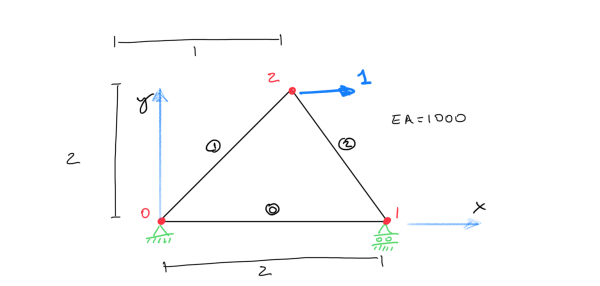
\includegraphics{esquema.png}
\caption{esquema}
\end{figure}

Como en el lenguaje python los arrays, listas, etc. se indexan empezando
por cero, uilizaremos ese convenio en la descripción del modelo. Los
nodos se numerarán de forma correlativa empezando por cero, con los
elementos se hará de forma similar y para establecer las fuerzas
concentradas en nodos se usará el nodo, la dirección (0 el eje x y 1 el
eje y) y el valor. Las condiciones de contorno se definirán de forma
similar a las fuerzas pero sin el dato valor. Si resumimos la
información del modelo relevante para el cálculo observamos lo
siguiente:

\begin{itemize}
\tightlist
\item
  Coordenadas de los nodos.
\end{itemize}

\begin{longtable}[]{@{}lll@{}}
\toprule
Nodo & x & y\tabularnewline
\midrule
\endhead
0 & 0 & 0\tabularnewline
1 & 2 & 0\tabularnewline
2 & 1 & 0\tabularnewline
\bottomrule
\end{longtable}

\begin{itemize}
\tightlist
\item
  Elementos (barras articuladas)
\end{itemize}

\begin{longtable}[]{@{}llll@{}}
\toprule
Elemento & nodo 1 & nodo 2 & EA\tabularnewline
\midrule
\endhead
0 & 0 & 1 & 1000\tabularnewline
1 & 0 & 2 & 1000\tabularnewline
2 & 1 & 2 & 1000\tabularnewline
\bottomrule
\end{longtable}

\begin{itemize}
\tightlist
\item
  fuerzas aplicadas
\end{itemize}

\begin{longtable}[]{@{}lll@{}}
\toprule
Nodo & dirección & valor\tabularnewline
\midrule
\endhead
2 & 0 & 1\tabularnewline
\bottomrule
\end{longtable}

\begin{itemize}
\tightlist
\item
  Condiciones de contorno
\end{itemize}

\begin{longtable}[]{@{}ll@{}}
\toprule
Nodo & dirección\tabularnewline
\midrule
\endhead
0 & 0\tabularnewline
0 & 1\tabularnewline
1 & 1\tabularnewline
\bottomrule
\end{longtable}

Lo primero que se hará es definir formalmente el modelo en el lenguaje
en cuestión. Para el caso que nos ocupa usaremos un array del tipo numpy
para las coordenadas y listas para los elementos, las fuerzas y las
condiciones de contorno. Crearemos las variables correspondientes con
los nombres que nos parezcan oportunos.

    Para los nodos un array con sus coordenadas
{[}{[}x0,y0{]},{[}x1,y1{]},\ldots{]}\\
Para los elementos una lista con los mismos {[}el1,el2,\ldots.{]}, donde
cada elemento es {[}nodo 1, nodo 2, EA{]}\\
Para las fuerzas una lista con cada una de las componentes
{[}{[}nodo,dirección,F\_val{]},\ldots{]}\\
Y para las condiciones de contorno una lista
similar{[}{[}nodo,dirección{]},\ldots{]}\\
Escribiéndolo en python tendríamos lo siguiente

    \begin{tcolorbox}[breakable, size=fbox, boxrule=1pt, pad at break*=1mm,colback=cellbackground, colframe=cellborder]
\prompt{In}{incolor}{2}{\boxspacing}
\begin{Verbatim}[commandchars=\\\{\}]
\PY{n}{x} \PY{o}{=} \PY{n}{np}\PY{o}{.}\PY{n}{array}\PY{p}{(}\PY{p}{[}\PY{p}{[}\PY{l+m+mi}{0}\PY{p}{,}\PY{l+m+mi}{0}\PY{p}{]}\PY{p}{,}\PY{p}{[}\PY{l+m+mi}{2}\PY{p}{,}\PY{l+m+mi}{0}\PY{p}{]}\PY{p}{,}\PY{p}{[}\PY{l+m+mi}{1}\PY{p}{,}\PY{l+m+mi}{2}\PY{p}{]}\PY{p}{]}\PY{p}{)}
\PY{n}{elementos} \PY{o}{=} \PY{p}{[}\PY{p}{[}\PY{l+m+mi}{0}\PY{p}{,}\PY{l+m+mi}{1}\PY{p}{,}\PY{l+m+mi}{1000}\PY{p}{]}\PY{p}{,}\PY{p}{[}\PY{l+m+mi}{0}\PY{p}{,}\PY{l+m+mi}{2}\PY{p}{,}\PY{l+m+mi}{1000}\PY{p}{]}\PY{p}{,}\PY{p}{[}\PY{l+m+mi}{1}\PY{p}{,}\PY{l+m+mi}{2}\PY{p}{,}\PY{l+m+mi}{1000}\PY{p}{]}\PY{p}{]}
\PY{n}{fuerzas} \PY{o}{=} \PY{p}{[}\PY{p}{[}\PY{l+m+mi}{2}\PY{p}{,}\PY{l+m+mi}{0}\PY{p}{,}\PY{l+m+mi}{1}\PY{p}{]}\PY{p}{]}
\PY{n}{cc} \PY{o}{=} \PY{p}{[}\PY{p}{[}\PY{l+m+mi}{0}\PY{p}{,}\PY{l+m+mi}{0}\PY{p}{]}\PY{p}{,}\PY{p}{[}\PY{l+m+mi}{0}\PY{p}{,}\PY{l+m+mi}{1}\PY{p}{]}\PY{p}{,}\PY{p}{[}\PY{l+m+mi}{1}\PY{p}{,}\PY{l+m+mi}{1}\PY{p}{]}\PY{p}{]}
\end{Verbatim}
\end{tcolorbox}

    \hypertarget{matriz-de-rigidez-del-modelo}{%
\subsection{Matriz de rigidez del
modelo}\label{matriz-de-rigidez-del-modelo}}

El objetivo del cálculo es llegar a una ecuación del tipo
$\mathbf{K}\mathbf{d}=\mathbf{f}$ donde $\mathbf{K}$ es la matriz de
rigidez global del modelo que se obtiene a partir de las matrices de
rigidez de cada elemento ensambladas (sumadas en una cierta posición
dependiente de los nodos) en la global.

El vector de fuerzas $\mathbf{f}$ también se obtiene de forma similar
ensamblando las fuerzas dadas cada una de ellas en la posición
correspondiente.

Como los grados de libertad considerados son dos por nodo (u según x,v
según y) las dimensiones de las matrices serán, siendo $n$ el número
de nodos.

\begin{longtable}[]{@{}ll@{}}
\toprule
Matriz & dimensión\tabularnewline
\midrule
\endhead
$\mathbf{K}$ & $2n\times 2n$\tabularnewline
$\mathbf{d}$ & $2n$\tabularnewline
$\mathbf{f}$ & $2n$\tabularnewline
\bottomrule
\end{longtable}

Al haber indexado a partir de cero la relación entre nodo, dirección y
grado de libertad es muy sencilla: Al nodo $i$, dirección $j$ le
corresonde el grado de libertad (índice en las matrices) $2i+j$

    \hypertarget{matriz-de-rigidez-elemental}{%
\subsection{Matriz de rigidez
elemental}\label{matriz-de-rigidez-elemental}}

Primeramente obtendremos la función matriz de rigidez de un elemento.
Una vez obtenida se aplicará esa función a todos los elementos y se
ensamblarán.

\begin{figure}
\centering
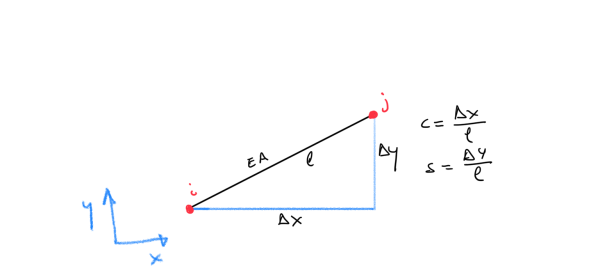
\includegraphics{elemento.png}
\caption{elemento}
\end{figure}

La matriz de rigidez del elemento es:

$ \mathbf{K}\_\{el\} = \frac{EA}{l}
\begin{pmatrix}
c^2 & cs & -c^2 & -cs \\
cs  & s^2 & cs & s^2 \\
-c^2 & -cs & c^2 & cs \\
-cs &  -s^2 & cs & s^2
\end{pmatrix}
$ 
siendo $c$ el coseno del ángulo que forma la barra con la
horizontal y $s$ el seno.

Como se puede observar, en este caso, está formada por un bloque de
$2\times2$ que se repite cuatro veces, dos de ellas con el signo
cambiado.

Si denominamos al bloque básico $\mathbf{K}_{11}$ tendríamos lo
siguiente $ \mathbf{K_{11}} = \frac{EA}{l}
\begin{pmatrix}
c^2 & cs \\
cs & s^2 
\end{pmatrix}
$

y por tanto: $ \mathbf{K_{el}} =
\begin{pmatrix}
\mathbf{K}_{11} & -\mathbf{K}_{11} \\
-\mathbf{K}_{11}& \mathbf{K}_{11} 
\end{pmatrix}
$

Vamos a proceder paso a paso escribiendo funciones para obtener la
matriz de rigidez elemental. Partimos de un elemento que está definido
por: {[}nodo 1,nodo 2, EA{]}.\\
Además necesitaremos las coordenadas de los nodos (en concreto las
diferencias) para obtener la longitud y los senos y los cosenos.

    La primera función que vamos incluir es la que accede a las coordenadas
de los nodos.\\
Argumentos: 1. elemento,coordenadas\\
{[}nodo 1,nodo 2, EA{]} , coordenadas\\
Resultado: 1. elemento modificado\\
{[}nodo 1, nodo 2, EA,x2-x1,y2-y1{]}

    \begin{tcolorbox}[breakable, size=fbox, boxrule=1pt, pad at break*=1mm,colback=cellbackground, colframe=cellborder]
\prompt{In}{incolor}{3}{\boxspacing}
\begin{Verbatim}[commandchars=\\\{\}]
\PY{n}{fk\PYZus{}0} \PY{o}{=} \PY{k}{lambda} \PY{n}{el}\PY{p}{,}\PY{n}{coor}\PY{p}{:} \PY{p}{[}\PY{n}{el}\PY{p}{[}\PY{l+m+mi}{0}\PY{p}{]}\PY{p}{,}\PY{n}{el}\PY{p}{[}\PY{l+m+mi}{1}\PY{p}{]}\PY{p}{,}\PY{n}{el}\PY{p}{[}\PY{l+m+mi}{2}\PY{p}{]}\PY{p}{,}\PY{n}{coor}\PY{p}{[}\PY{n}{el}\PY{p}{[}\PY{l+m+mi}{1}\PY{p}{]}\PY{p}{]}\PY{p}{[}\PY{l+m+mi}{0}\PY{p}{]}\PY{o}{\PYZhy{}}\PY{n}{coor}\PY{p}{[}\PY{n}{el}\PY{p}{[}\PY{l+m+mi}{0}\PY{p}{]}\PY{p}{]}\PY{p}{[}\PY{l+m+mi}{0}\PY{p}{]}\PY{p}{,}\PY{n}{coor}\PY{p}{[}\PY{n}{el}\PY{p}{[}\PY{l+m+mi}{1}\PY{p}{]}\PY{p}{]}\PY{p}{[}\PY{l+m+mi}{1}\PY{p}{]}\PY{o}{\PYZhy{}}\PY{n}{coor}\PY{p}{[}\PY{n}{el}\PY{p}{[}\PY{l+m+mi}{0}\PY{p}{]}\PY{p}{]}\PY{p}{[}\PY{l+m+mi}{1}\PY{p}{]}\PY{p}{]}
\end{Verbatim}
\end{tcolorbox}

    Para aplicar la función al elemento número 1 (elementos{[}1{]}) se haría
del siguiente modo:

    \begin{tcolorbox}[breakable, size=fbox, boxrule=1pt, pad at break*=1mm,colback=cellbackground, colframe=cellborder]
\prompt{In}{incolor}{4}{\boxspacing}
\begin{Verbatim}[commandchars=\\\{\}]
\PY{n}{fk\PYZus{}0}\PY{p}{(}\PY{n}{elementos}\PY{p}{[}\PY{l+m+mi}{1}\PY{p}{]}\PY{p}{,}\PY{n}{x}\PY{p}{)}
\end{Verbatim}
\end{tcolorbox}

            \begin{tcolorbox}[breakable, size=fbox, boxrule=.5pt, pad at break*=1mm, opacityfill=0]
\prompt{Out}{outcolor}{4}{\boxspacing}
\begin{Verbatim}[commandchars=\\\{\}]
[0, 2, 1000, 1, 2]
\end{Verbatim}
\end{tcolorbox}
        
    La siguiente función calcula la longitud del elemento\\
Argumentos:\\
1. elemento\\
{[}nodo 1,nodo 2, EA,x2-x1,y2-y1{]}\\
Resultado:\\
1. elemento modificado\\
{[}nodo 1, nodo 2, EA,l,x2-x1,y2-y1{]}

    \begin{tcolorbox}[breakable, size=fbox, boxrule=1pt, pad at break*=1mm,colback=cellbackground, colframe=cellborder]
\prompt{In}{incolor}{5}{\boxspacing}
\begin{Verbatim}[commandchars=\\\{\}]
\PY{n}{fk\PYZus{}1} \PY{o}{=} \PY{k}{lambda} \PY{n}{el}\PY{p}{:} \PY{p}{[}\PY{n}{el}\PY{p}{[}\PY{l+m+mi}{0}\PY{p}{]}\PY{p}{,}\PY{n}{el}\PY{p}{[}\PY{l+m+mi}{1}\PY{p}{]}\PY{p}{,}\PY{n}{el}\PY{p}{[}\PY{l+m+mi}{2}\PY{p}{]}\PY{p}{,}\PY{n}{math}\PY{o}{.}\PY{n}{hypot}\PY{p}{(}\PY{n}{el}\PY{p}{[}\PY{l+m+mi}{3}\PY{p}{]}\PY{p}{,}\PY{n}{el}\PY{p}{[}\PY{l+m+mi}{4}\PY{p}{]}\PY{p}{)}\PY{p}{,}\PY{n}{el}\PY{p}{[}\PY{l+m+mi}{3}\PY{p}{]}\PY{p}{,}\PY{n}{el}\PY{p}{[}\PY{l+m+mi}{4}\PY{p}{]}\PY{p}{]}
\end{Verbatim}
\end{tcolorbox}

    Vemos como se aplicaría al elemento cero.

    \begin{tcolorbox}[breakable, size=fbox, boxrule=1pt, pad at break*=1mm,colback=cellbackground, colframe=cellborder]
\prompt{In}{incolor}{6}{\boxspacing}
\begin{Verbatim}[commandchars=\\\{\}]
\PY{n}{fk\PYZus{}0}\PY{p}{(}\PY{n}{elementos}\PY{p}{[}\PY{l+m+mi}{0}\PY{p}{]}\PY{p}{,}\PY{n}{x}\PY{p}{)}
\PY{n}{fk\PYZus{}1}\PY{p}{(}\PY{n}{fk\PYZus{}0}\PY{p}{(}\PY{n}{elementos}\PY{p}{[}\PY{l+m+mi}{0}\PY{p}{]}\PY{p}{,}\PY{n}{x}\PY{p}{)}\PY{p}{)}
\end{Verbatim}
\end{tcolorbox}

            \begin{tcolorbox}[breakable, size=fbox, boxrule=.5pt, pad at break*=1mm, opacityfill=0]
\prompt{Out}{outcolor}{6}{\boxspacing}
\begin{Verbatim}[commandchars=\\\{\}]
[0, 1, 1000, 2.0, 2, 0]
\end{Verbatim}
\end{tcolorbox}
        
    Una vez que tenemos la longitud y las diferencias de coordenadas se
puede obtener el coseno y el seno y la rigidez axial $\frac{EA}{l}$
del elemento donde tanto el coseno como el seno se obtienen a partir de
las diferencias de coordenadas y de la longitud.\\
Se hace mediante una nueva función \textbf{fk\_2}

    \begin{tcolorbox}[breakable, size=fbox, boxrule=1pt, pad at break*=1mm,colback=cellbackground, colframe=cellborder]
\prompt{In}{incolor}{7}{\boxspacing}
\begin{Verbatim}[commandchars=\\\{\}]
\PY{n}{fk\PYZus{}2} \PY{o}{=} \PY{k}{lambda} \PY{n}{el}\PY{p}{:} \PY{p}{[}\PY{n}{el}\PY{p}{[}\PY{l+m+mi}{0}\PY{p}{]}\PY{p}{,}\PY{n}{el}\PY{p}{[}\PY{l+m+mi}{1}\PY{p}{]}\PY{p}{,}\PY{n}{el}\PY{p}{[}\PY{l+m+mi}{2}\PY{p}{]}\PY{o}{/}\PY{n}{el}\PY{p}{[}\PY{l+m+mi}{3}\PY{p}{]}\PY{p}{,}\PY{n}{el}\PY{p}{[}\PY{l+m+mi}{4}\PY{p}{]}\PY{o}{/}\PY{n}{el}\PY{p}{[}\PY{l+m+mi}{3}\PY{p}{]}\PY{p}{,}\PY{n}{el}\PY{p}{[}\PY{l+m+mi}{5}\PY{p}{]}\PY{o}{/}\PY{n}{el}\PY{p}{[}\PY{l+m+mi}{3}\PY{p}{]}\PY{p}{]}
\end{Verbatim}
\end{tcolorbox}

    Obsérvese que cada función parte de los resultados de la función
anterior.

    \begin{tcolorbox}[breakable, size=fbox, boxrule=1pt, pad at break*=1mm,colback=cellbackground, colframe=cellborder]
\prompt{In}{incolor}{8}{\boxspacing}
\begin{Verbatim}[commandchars=\\\{\}]
\PY{n}{fk\PYZus{}0}\PY{p}{(}\PY{n}{elementos}\PY{p}{[}\PY{l+m+mi}{0}\PY{p}{]}\PY{p}{,}\PY{n}{x}\PY{p}{)}
\PY{n}{fk\PYZus{}1}\PY{p}{(}\PY{n}{fk\PYZus{}0}\PY{p}{(}\PY{n}{elementos}\PY{p}{[}\PY{l+m+mi}{0}\PY{p}{]}\PY{p}{,}\PY{n}{x}\PY{p}{)}\PY{p}{)}
\PY{n}{fk\PYZus{}2}\PY{p}{(}\PY{n}{fk\PYZus{}1}\PY{p}{(}\PY{n}{fk\PYZus{}0}\PY{p}{(}\PY{n}{elementos}\PY{p}{[}\PY{l+m+mi}{0}\PY{p}{]}\PY{p}{,}\PY{n}{x}\PY{p}{)}\PY{p}{)}\PY{p}{)}
\end{Verbatim}
\end{tcolorbox}

            \begin{tcolorbox}[breakable, size=fbox, boxrule=.5pt, pad at break*=1mm, opacityfill=0]
\prompt{Out}{outcolor}{8}{\boxspacing}
\begin{Verbatim}[commandchars=\\\{\}]
[0, 1, 500.0, 1.0, 0.0]
\end{Verbatim}
\end{tcolorbox}
        
    Ahora se puede obtener el bloque elemental $\mathbf{K}_{11}$ de la
matriz de rigidez elemental\\
$ \mathbf{K_{11}} = \frac{EA}{l}
\begin{pmatrix}
c^2 & cs \\
cs & s^2 
\end{pmatrix}
$

    \begin{tcolorbox}[breakable, size=fbox, boxrule=1pt, pad at break*=1mm,colback=cellbackground, colframe=cellborder]
\prompt{In}{incolor}{9}{\boxspacing}
\begin{Verbatim}[commandchars=\\\{\}]
\PY{n}{fk\PYZus{}11} \PY{o}{=} \PY{k}{lambda} \PY{n}{el}\PY{p}{:} \PY{n}{el}\PY{p}{[}\PY{l+m+mi}{2}\PY{p}{]}\PY{o}{*}\PY{n}{np}\PY{o}{.}\PY{n}{array}\PY{p}{(}\PY{p}{[}\PY{p}{[}\PY{n}{el}\PY{p}{[}\PY{l+m+mi}{3}\PY{p}{]}\PY{o}{*}\PY{o}{*}\PY{l+m+mi}{2}\PY{p}{,}\PY{n}{el}\PY{p}{[}\PY{l+m+mi}{3}\PY{p}{]}\PY{o}{*}\PY{n}{el}\PY{p}{[}\PY{l+m+mi}{4}\PY{p}{]}\PY{p}{]}\PY{p}{,}\PY{p}{[}\PY{n}{el}\PY{p}{[}\PY{l+m+mi}{3}\PY{p}{]}\PY{o}{*}\PY{n}{el}\PY{p}{[}\PY{l+m+mi}{4}\PY{p}{]}\PY{p}{,}\PY{n}{el}\PY{p}{[}\PY{l+m+mi}{4}\PY{p}{]}\PY{o}{*}\PY{o}{*}\PY{l+m+mi}{2}\PY{p}{]}\PY{p}{]}\PY{p}{)}
\end{Verbatim}
\end{tcolorbox}

    El bloque elemental es un array del tipo numpy.

    \begin{tcolorbox}[breakable, size=fbox, boxrule=1pt, pad at break*=1mm,colback=cellbackground, colframe=cellborder]
\prompt{In}{incolor}{10}{\boxspacing}
\begin{Verbatim}[commandchars=\\\{\}]
\PY{n}{fk\PYZus{}11}\PY{p}{(}\PY{n}{fk\PYZus{}2}\PY{p}{(}\PY{n}{fk\PYZus{}1}\PY{p}{(}\PY{n}{fk\PYZus{}0}\PY{p}{(}\PY{n}{elementos}\PY{p}{[}\PY{l+m+mi}{0}\PY{p}{]}\PY{p}{,}\PY{n}{x}\PY{p}{)}\PY{p}{)}\PY{p}{)}\PY{p}{)}
\end{Verbatim}
\end{tcolorbox}

            \begin{tcolorbox}[breakable, size=fbox, boxrule=.5pt, pad at break*=1mm, opacityfill=0]
\prompt{Out}{outcolor}{10}{\boxspacing}
\begin{Verbatim}[commandchars=\\\{\}]
array([[500.,   0.],
       [  0.,   0.]])
\end{Verbatim}
\end{tcolorbox}
        
    \begin{center}\rule{0.5\linewidth}{0.5pt}\end{center}

Y a partir del bloque $\mathbf{K}_{11}$ podemos obtener la matriz de
rigidez local del elemento\\
$ \mathbf{K_{el}} =
\begin{pmatrix}
\mathbf{K}_{11} & -\mathbf{K}_{11} \\
-\mathbf{K}_{11}& \mathbf{K}_{11} 
\end{pmatrix}
$

    \begin{tcolorbox}[breakable, size=fbox, boxrule=1pt, pad at break*=1mm,colback=cellbackground, colframe=cellborder]
\prompt{In}{incolor}{11}{\boxspacing}
\begin{Verbatim}[commandchars=\\\{\}]
\PY{n}{fk\PYZus{}loc} \PY{o}{=} \PY{k}{lambda} \PY{n}{k11}\PY{p}{:} \PY{n}{np}\PY{o}{.}\PY{n}{vstack}\PY{p}{(}\PY{p}{(}\PY{n}{np}\PY{o}{.}\PY{n}{hstack}\PY{p}{(}\PY{p}{(}\PY{n}{k11}\PY{p}{,}\PY{o}{\PYZhy{}}\PY{n}{k11}\PY{p}{)}\PY{p}{)}\PY{p}{,}\PY{n}{np}\PY{o}{.}\PY{n}{hstack}\PY{p}{(}\PY{p}{(}\PY{o}{\PYZhy{}}\PY{n}{k11}\PY{p}{,}\PY{n}{k11}\PY{p}{)}\PY{p}{)}\PY{p}{)}\PY{p}{)}
\end{Verbatim}
\end{tcolorbox}

    \begin{tcolorbox}[breakable, size=fbox, boxrule=1pt, pad at break*=1mm,colback=cellbackground, colframe=cellborder]
\prompt{In}{incolor}{12}{\boxspacing}
\begin{Verbatim}[commandchars=\\\{\}]
\PY{n}{fk\PYZus{}loc}\PY{p}{(}\PY{n}{fk\PYZus{}11}\PY{p}{(}\PY{n}{fk\PYZus{}2}\PY{p}{(}\PY{n}{fk\PYZus{}1}\PY{p}{(}\PY{n}{fk\PYZus{}0}\PY{p}{(}\PY{n}{elementos}\PY{p}{[}\PY{l+m+mi}{0}\PY{p}{]}\PY{p}{,}\PY{n}{x}\PY{p}{)}\PY{p}{)}\PY{p}{)}\PY{p}{)}\PY{p}{)}
\end{Verbatim}
\end{tcolorbox}

            \begin{tcolorbox}[breakable, size=fbox, boxrule=.5pt, pad at break*=1mm, opacityfill=0]
\prompt{Out}{outcolor}{12}{\boxspacing}
\begin{Verbatim}[commandchars=\\\{\}]
array([[ 500.,    0., -500.,   -0.],
       [   0.,    0.,   -0.,   -0.],
       [-500.,   -0.,  500.,    0.],
       [  -0.,   -0.,    0.,    0.]])
\end{Verbatim}
\end{tcolorbox}
        
    Todas las funciones auxiliares para obtener la matriz de rigidez las
podemos juntar en una sola que a partir de los datos de un elemento y
del array de coordenadas del modelo devuelve la matriz de rigidez del
elemento.

    \begin{tcolorbox}[breakable, size=fbox, boxrule=1pt, pad at break*=1mm,colback=cellbackground, colframe=cellborder]
\prompt{In}{incolor}{13}{\boxspacing}
\begin{Verbatim}[commandchars=\\\{\}]
\PY{n}{fk\PYZus{}el} \PY{o}{=} \PY{k}{lambda} \PY{n}{elemento}\PY{p}{,}\PY{n}{coor}\PY{p}{:} \PY{n}{fk\PYZus{}loc}\PY{p}{(}\PY{n}{fk\PYZus{}11}\PY{p}{(}\PY{n}{fk\PYZus{}2}\PY{p}{(}\PY{n}{fk\PYZus{}1}\PY{p}{(}\PY{n}{fk\PYZus{}0}\PY{p}{(}\PY{n}{elemento}\PY{p}{,}\PY{n}{coor}\PY{p}{)}\PY{p}{)}\PY{p}{)}\PY{p}{)}\PY{p}{)}
\end{Verbatim}
\end{tcolorbox}

    \begin{tcolorbox}[breakable, size=fbox, boxrule=1pt, pad at break*=1mm,colback=cellbackground, colframe=cellborder]
\prompt{In}{incolor}{14}{\boxspacing}
\begin{Verbatim}[commandchars=\\\{\}]
\PY{n}{fk\PYZus{}el}\PY{p}{(}\PY{n}{elementos}\PY{p}{[}\PY{l+m+mi}{2}\PY{p}{]}\PY{p}{,}\PY{n}{x}\PY{p}{)}
\end{Verbatim}
\end{tcolorbox}

            \begin{tcolorbox}[breakable, size=fbox, boxrule=.5pt, pad at break*=1mm, opacityfill=0]
\prompt{Out}{outcolor}{14}{\boxspacing}
\begin{Verbatim}[commandchars=\\\{\}]
array([[  89.4427191, -178.8854382,  -89.4427191,  178.8854382],
       [-178.8854382,  357.7708764,  178.8854382, -357.7708764],
       [ -89.4427191,  178.8854382,   89.4427191, -178.8854382],
       [ 178.8854382, -357.7708764, -178.8854382,  357.7708764]])
\end{Verbatim}
\end{tcolorbox}
        
    \hypertarget{matriz-de-rigidez-de-un-conjunto-de-elementos-y-ensamblaje}{%
\subsection{Matriz de rigidez de un conjunto de elementos y
ensamblaje}\label{matriz-de-rigidez-de-un-conjunto-de-elementos-y-ensamblaje}}

Una vez que tengo una función para obtener la matriz de rigidez de un
elemento, la forma de obtener las matrices de rigidez de todos los
elementos es aplicar esa función a todos los elementos.

    \begin{tcolorbox}[breakable, size=fbox, boxrule=1pt, pad at break*=1mm,colback=cellbackground, colframe=cellborder]
\prompt{In}{incolor}{15}{\boxspacing}
\begin{Verbatim}[commandchars=\\\{\}]
\PY{n}{fk\PYZus{}els} \PY{o}{=} \PY{k}{lambda} \PY{n}{elementos}\PY{p}{,}\PY{n}{coor}\PY{p}{:} \PY{n+nb}{list}\PY{p}{(}\PY{n+nb}{map}\PY{p}{(}\PY{k}{lambda} \PY{n}{elemento}\PY{p}{:} \PY{n}{fk\PYZus{}el}\PY{p}{(}\PY{n}{elemento}\PY{p}{,}\PY{n}{coor}\PY{p}{)}\PY{p}{,}\PY{n}{elementos}\PY{p}{)}\PY{p}{)}
\end{Verbatim}
\end{tcolorbox}

    \begin{tcolorbox}[breakable, size=fbox, boxrule=1pt, pad at break*=1mm,colback=cellbackground, colframe=cellborder]
\prompt{In}{incolor}{16}{\boxspacing}
\begin{Verbatim}[commandchars=\\\{\}]
\PY{n}{fk\PYZus{}els}\PY{p}{(}\PY{n}{elementos}\PY{p}{,}\PY{n}{x}\PY{p}{)}
\end{Verbatim}
\end{tcolorbox}

            \begin{tcolorbox}[breakable, size=fbox, boxrule=.5pt, pad at break*=1mm, opacityfill=0]
\prompt{Out}{outcolor}{16}{\boxspacing}
\begin{Verbatim}[commandchars=\\\{\}]
[array([[ 500.,    0., -500.,   -0.],
        [   0.,    0.,   -0.,   -0.],
        [-500.,   -0.,  500.,    0.],
        [  -0.,   -0.,    0.,    0.]]),
 array([[  89.4427191,  178.8854382,  -89.4427191, -178.8854382],
        [ 178.8854382,  357.7708764, -178.8854382, -357.7708764],
        [ -89.4427191, -178.8854382,   89.4427191,  178.8854382],
        [-178.8854382, -357.7708764,  178.8854382,  357.7708764]]),
 array([[  89.4427191, -178.8854382,  -89.4427191,  178.8854382],
        [-178.8854382,  357.7708764,  178.8854382, -357.7708764],
        [ -89.4427191,  178.8854382,   89.4427191, -178.8854382],
        [ 178.8854382, -357.7708764, -178.8854382,  357.7708764]])]
\end{Verbatim}
\end{tcolorbox}
        
    Con vistas al ensamblaje nos conviene tener todos los elementos de las
matrices de rigidez en un array unidimensional. Para ello usaremos la
función np.ravel y definimos una nueva función.\\
Esta función simplemeente calcula todas las matrices de rigidez de todos
los elementos y las devuelve en un array de una dimensión.

    \begin{tcolorbox}[breakable, size=fbox, boxrule=1pt, pad at break*=1mm,colback=cellbackground, colframe=cellborder]
\prompt{In}{incolor}{17}{\boxspacing}
\begin{Verbatim}[commandchars=\\\{\}]
\PY{n}{f\PYZus{}kg1} \PY{o}{=} \PY{k}{lambda} \PY{n}{elementos}\PY{p}{,}\PY{n}{coordenadas}\PY{p}{:}\PY{n}{np}\PY{o}{.}\PY{n}{ravel}\PY{p}{(}\PY{n}{fk\PYZus{}els}\PY{p}{(}\PY{n}{elementos}\PY{p}{,}\PY{n}{coordenadas}\PY{p}{)}\PY{p}{)}
\end{Verbatim}
\end{tcolorbox}

    \begin{tcolorbox}[breakable, size=fbox, boxrule=1pt, pad at break*=1mm,colback=cellbackground, colframe=cellborder]
\prompt{In}{incolor}{18}{\boxspacing}
\begin{Verbatim}[commandchars=\\\{\}]
\PY{n}{f\PYZus{}kg1}\PY{p}{(}\PY{n}{elementos}\PY{p}{,}\PY{n}{x}\PY{p}{)}
\end{Verbatim}
\end{tcolorbox}

            \begin{tcolorbox}[breakable, size=fbox, boxrule=.5pt, pad at break*=1mm, opacityfill=0]
\prompt{Out}{outcolor}{18}{\boxspacing}
\begin{Verbatim}[commandchars=\\\{\}]
array([ 500.       ,    0.       , -500.       ,   -0.       ,
          0.       ,    0.       ,   -0.       ,   -0.       ,
       -500.       ,   -0.       ,  500.       ,    0.       ,
         -0.       ,   -0.       ,    0.       ,    0.       ,
         89.4427191,  178.8854382,  -89.4427191, -178.8854382,
        178.8854382,  357.7708764, -178.8854382, -357.7708764,
        -89.4427191, -178.8854382,   89.4427191,  178.8854382,
       -178.8854382, -357.7708764,  178.8854382,  357.7708764,
         89.4427191, -178.8854382,  -89.4427191,  178.8854382,
       -178.8854382,  357.7708764,  178.8854382, -357.7708764,
        -89.4427191,  178.8854382,   89.4427191, -178.8854382,
        178.8854382, -357.7708764, -178.8854382,  357.7708764])
\end{Verbatim}
\end{tcolorbox}
        
    Para poder enamblar las matrices de rigidez es necesario saber a que
índices de la matriz de rigidez global va cada elemento de una matriz de
rigidez elemental. Vamos a crear unas funciones que nos den esos índices
en función de los nodos del elemento, una función para las filas de
todos los elementos de la matriz y otra función para las columnas.

    \begin{tcolorbox}[breakable, size=fbox, boxrule=1pt, pad at break*=1mm,colback=cellbackground, colframe=cellborder]
\prompt{In}{incolor}{19}{\boxspacing}
\begin{Verbatim}[commandchars=\\\{\}]
\PY{n}{columnask} \PY{o}{=} \PY{k}{lambda} \PY{n}{y}\PY{p}{:}  \PY{n}{np}\PY{o}{.}\PY{n}{array}\PY{p}{(}\PY{n+nb}{list}\PY{p}{(}\PY{p}{(} \PY{n+nb}{map}\PY{p}{(}\PY{k}{lambda} \PY{n}{x}\PY{p}{:} \PY{p}{[}\PY{n}{x}\PY{o}{*}\PY{l+m+mi}{2}\PY{p}{,}\PY{n}{x}\PY{o}{*}\PY{l+m+mi}{2}\PY{o}{+}\PY{l+m+mi}{1}\PY{p}{]}\PY{p}{,}\PY{n}{y}\PY{p}{)}\PY{p}{)}\PY{p}{)}\PY{o}{*}\PY{l+m+mi}{4}\PY{p}{)}\PY{o}{.}\PY{n}{flatten}\PY{p}{(}\PY{p}{)}
\PY{n}{filask} \PY{o}{=} \PY{k}{lambda} \PY{n}{y}\PY{p}{:}  \PY{n}{np}\PY{o}{.}\PY{n}{array}\PY{p}{(}\PY{n+nb}{list}\PY{p}{(}\PY{p}{(} \PY{n+nb}{map}\PY{p}{(}\PY{k}{lambda} \PY{n}{x}\PY{p}{:} \PY{p}{[}\PY{n+nb}{list}\PY{p}{(}\PY{p}{[}\PY{n}{x}\PY{o}{*}\PY{l+m+mi}{2}\PY{p}{]}\PY{p}{)}\PY{o}{*}\PY{l+m+mi}{4}\PY{p}{,}\PY{n+nb}{list}\PY{p}{(}\PY{p}{[}\PY{n}{x}\PY{o}{*}\PY{l+m+mi}{2}\PY{o}{+}\PY{l+m+mi}{1}\PY{p}{]}\PY{p}{)}\PY{o}{*}\PY{l+m+mi}{4}\PY{p}{]}\PY{p}{,}\PY{n}{y}\PY{p}{)}\PY{p}{)}\PY{p}{)}\PY{p}{)}\PY{o}{.}\PY{n}{flatten}\PY{p}{(}\PY{p}{)}
\end{Verbatim}
\end{tcolorbox}

    Si se desea saber a que filas de la matriz de rigidez global van los
elementos de la matriz de rigidez del elemento que une los nodos $0$ y
$1$ usaríamos la función filask((0,1)).\\
Del mismo modo para las columnas de la matriz de rigidez del elemento
que va del nodo $1$ al nodo $2$ las columnas serían
columnask((1,2)).

    \begin{tcolorbox}[breakable, size=fbox, boxrule=1pt, pad at break*=1mm,colback=cellbackground, colframe=cellborder]
\prompt{In}{incolor}{20}{\boxspacing}
\begin{Verbatim}[commandchars=\\\{\}]
\PY{n+nb}{print}\PY{p}{(}\PY{n}{filask}\PY{p}{(}\PY{p}{(}\PY{l+m+mi}{0}\PY{p}{,}\PY{l+m+mi}{1}\PY{p}{)}\PY{p}{)}\PY{p}{)}
\PY{n+nb}{print}\PY{p}{(}\PY{n}{columnask}\PY{p}{(}\PY{p}{(}\PY{l+m+mi}{1}\PY{p}{,}\PY{l+m+mi}{2}\PY{p}{)}\PY{p}{)}\PY{p}{)}
\end{Verbatim}
\end{tcolorbox}

    \begin{Verbatim}[commandchars=\\\{\}]
[0 0 0 0 1 1 1 1 2 2 2 2 3 3 3 3]
[2 3 4 5 2 3 4 5 2 3 4 5 2 3 4 5]
    \end{Verbatim}

    Si se aplican las funciones a un conjunto de elementos se definen las
siguientes funciones

    \begin{tcolorbox}[breakable, size=fbox, boxrule=1pt, pad at break*=1mm,colback=cellbackground, colframe=cellborder]
\prompt{In}{incolor}{21}{\boxspacing}
\begin{Verbatim}[commandchars=\\\{\}]
\PY{n}{fco} \PY{o}{=} \PY{k}{lambda} \PY{n}{elementos}\PY{p}{:} \PY{n+nb}{list}\PY{p}{(}\PY{n}{np}\PY{o}{.}\PY{n}{ravel}\PY{p}{(}\PY{n+nb}{list}\PY{p}{(}\PY{n+nb}{map}\PY{p}{(}\PY{k}{lambda} \PY{n}{u}\PY{p}{:} \PY{n}{columnask}\PY{p}{(}\PY{p}{(}\PY{n}{u}\PY{p}{[}\PY{l+m+mi}{0}\PY{p}{]}\PY{p}{,}\PY{n}{u}\PY{p}{[}\PY{l+m+mi}{1}\PY{p}{]}\PY{p}{)}\PY{p}{)}\PY{p}{,}\PY{n}{elementos}\PY{p}{)}\PY{p}{)}\PY{p}{)}\PY{p}{)}
\PY{n}{ffi} \PY{o}{=} \PY{k}{lambda} \PY{n}{elementos}\PY{p}{:} \PY{n+nb}{list}\PY{p}{(}\PY{n}{np}\PY{o}{.}\PY{n}{ravel}\PY{p}{(}\PY{n+nb}{list}\PY{p}{(}\PY{n+nb}{map}\PY{p}{(}\PY{k}{lambda} \PY{n}{u}\PY{p}{:} \PY{n}{filask}\PY{p}{(}\PY{p}{(}\PY{n}{u}\PY{p}{[}\PY{l+m+mi}{0}\PY{p}{]}\PY{p}{,}\PY{n}{u}\PY{p}{[}\PY{l+m+mi}{1}\PY{p}{]}\PY{p}{)}\PY{p}{)}\PY{p}{,}\PY{n}{elementos}\PY{p}{)}\PY{p}{)}\PY{p}{)}\PY{p}{)}
\end{Verbatim}
\end{tcolorbox}

    Como ejemplo oara obtener las columnas de todos los elementos de todas
las matrices de rigidez se ejecutaría \textbf{fco(elementos)}

    \begin{tcolorbox}[breakable, size=fbox, boxrule=1pt, pad at break*=1mm,colback=cellbackground, colframe=cellborder]
\prompt{In}{incolor}{22}{\boxspacing}
\begin{Verbatim}[commandchars=\\\{\}]
\PY{n+nb}{print}\PY{p}{(}\PY{n}{fco}\PY{p}{(}\PY{n}{elementos}\PY{p}{)}\PY{p}{)}
\end{Verbatim}
\end{tcolorbox}

    \begin{Verbatim}[commandchars=\\\{\}]
[0, 1, 2, 3, 0, 1, 2, 3, 0, 1, 2, 3, 0, 1, 2, 3, 0, 1, 4, 5, 0, 1, 4, 5, 0, 1,
4, 5, 0, 1, 4, 5, 2, 3, 4, 5, 2, 3, 4, 5, 2, 3, 4, 5, 2, 3, 4, 5]
    \end{Verbatim}

    Una vez que se dispone de las matrices de rigidez de todos los elementos
y las filas y columnas de cada elemento de cada matriz se pueden
ensamblar en la matriz de rigidez global. Utilizaremos el formato de
matriz sparse del módulo de python scipy que a la vez que genera la
matriz sparse va sumando los distintos elemntos.

    \begin{tcolorbox}[breakable, size=fbox, boxrule=1pt, pad at break*=1mm,colback=cellbackground, colframe=cellborder]
\prompt{In}{incolor}{23}{\boxspacing}
\begin{Verbatim}[commandchars=\\\{\}]
\PY{n}{f\PYZus{}kg} \PY{o}{=} \PY{k}{lambda} \PY{n}{elems}\PY{p}{,}\PY{n}{x}\PY{p}{:} \PY{n}{sp}\PY{o}{.}\PY{n}{csr\PYZus{}matrix}\PY{p}{(}\PY{n}{sp}\PY{o}{.}\PY{n}{coo\PYZus{}matrix}\PY{p}{(}\PY{p}{(}\PY{n}{f\PYZus{}kg1}\PY{p}{(}\PY{n}{elems}\PY{p}{,}\PY{n}{x}\PY{p}{)}\PY{p}{,}\PY{p}{(}\PY{n}{fco}\PY{p}{(}\PY{n}{elems}\PY{p}{)}\PY{p}{,}\PY{n}{ffi}\PY{p}{(}\PY{n}{elems}\PY{p}{)}\PY{p}{)}\PY{p}{)}\PY{p}{,}\PY{n}{shape}\PY{o}{=}\PY{p}{(}\PY{n+nb}{len}\PY{p}{(}\PY{n}{x}\PY{p}{)}\PY{o}{*}\PY{l+m+mi}{2}\PY{p}{,}\PY{n+nb}{len}\PY{p}{(}\PY{n}{x}\PY{p}{)}\PY{o}{*}\PY{l+m+mi}{2}\PY{p}{)}\PY{p}{)}\PY{p}{)}
\end{Verbatim}
\end{tcolorbox}

    La matriz obtenida es de tipo \emph{sparse}. Para poder escribirla en el
formato convencional se convierte a densa.

    \begin{tcolorbox}[breakable, size=fbox, boxrule=1pt, pad at break*=1mm,colback=cellbackground, colframe=cellborder]
\prompt{In}{incolor}{24}{\boxspacing}
\begin{Verbatim}[commandchars=\\\{\}]
\PY{n+nb}{print}\PY{p}{(}\PY{n}{f\PYZus{}kg}\PY{p}{(}\PY{n}{elementos}\PY{p}{,}\PY{n}{x}\PY{p}{)}\PY{o}{.}\PY{n}{todense}\PY{p}{(}\PY{p}{)}\PY{p}{)}
\end{Verbatim}
\end{tcolorbox}

    \begin{Verbatim}[commandchars=\\\{\}]
[[ 589.4427191  178.8854382 -500.           0.         -89.4427191
  -178.8854382]
 [ 178.8854382  357.7708764    0.           0.        -178.8854382
  -357.7708764]
 [-500.           0.         589.4427191 -178.8854382  -89.4427191
   178.8854382]
 [   0.           0.        -178.8854382  357.7708764  178.8854382
  -357.7708764]
 [ -89.4427191 -178.8854382  -89.4427191  178.8854382  178.8854382
     0.       ]
 [-178.8854382 -357.7708764  178.8854382 -357.7708764    0.
   715.5417528]]
    \end{Verbatim}

    \hypertarget{condiciones-de-contorno}{%
\subsection{Condiciones de contorno}\label{condiciones-de-contorno}}

La matriz obtenida es singular dado que no hemos incluido ninguna
condición de contorno.

    \begin{tcolorbox}[breakable, size=fbox, boxrule=1pt, pad at break*=1mm,colback=cellbackground, colframe=cellborder]
\prompt{In}{incolor}{25}{\boxspacing}
\begin{Verbatim}[commandchars=\\\{\}]
\PY{n}{np}\PY{o}{.}\PY{n}{linalg}\PY{o}{.}\PY{n}{det}\PY{p}{(}\PY{n}{f\PYZus{}kg}\PY{p}{(}\PY{n}{elementos}\PY{p}{,}\PY{n}{x}\PY{p}{)}\PY{o}{.}\PY{n}{todense}\PY{p}{(}\PY{p}{)}\PY{p}{)}
\end{Verbatim}
\end{tcolorbox}

            \begin{tcolorbox}[breakable, size=fbox, boxrule=.5pt, pad at break*=1mm, opacityfill=0]
\prompt{Out}{outcolor}{25}{\boxspacing}
\begin{Verbatim}[commandchars=\\\{\}]
0.0
\end{Verbatim}
\end{tcolorbox}
        
    Las condiciones de contorno podrían incluirse eliminando las filas y
columnas de la matriz de rigidez correspondientes a los grados de
libertad restringidos, pero una forma más simple es imponiendo las
restricciones por penalización. Se añaden en los elementos de la
diagonal de la matriz de rigidez correspondientes a los grados de
libertad restringidos unos valores de rigidez muy elevados que imponen
de forma aproximada el cumplimiento de la restricción.\\
De este modo se mantienen las dimensiones de las matrices que en el otro
caso habrían cambiado.

Si denominamos al valor elevado de rigidez $kpen$ y tenemos en el nodo
$i$ restringido el grado de libertad $j$ basta con añadir el valor
$kpen$ al elemento de la matriz de rigidez global
$\left(2i+j,2i+j\right)$

Para poder incluir estas condiciones de contorno de forma sencilla se
prepara una función \textbf{f\_kgp} que utiliza la matriz de rigidez
global y añade los elementos correspondientes (\textbf{f\_cc1} devuelve
el valor de los elementos y \textbf{f\_cc2} los índices fila y columna
de la matriz de rigidez global) en el sitio adecuado.

    \begin{tcolorbox}[breakable, size=fbox, boxrule=1pt, pad at break*=1mm,colback=cellbackground, colframe=cellborder]
\prompt{In}{incolor}{26}{\boxspacing}
\begin{Verbatim}[commandchars=\\\{\}]
\PY{n}{kpen} \PY{o}{=} \PY{l+m+mf}{1e20}
\PY{n}{f\PYZus{}cc1} \PY{o}{=} \PY{k}{lambda} \PY{n}{cc}\PY{p}{:} \PY{n+nb}{list}\PY{p}{(}\PY{n+nb}{map}\PY{p}{(}\PY{k}{lambda} \PY{n}{u}\PY{p}{:} \PY{n}{kpen}\PY{p}{,}\PY{n}{cc}\PY{p}{)}\PY{p}{)}
\PY{n}{f\PYZus{}cc2} \PY{o}{=} \PY{k}{lambda} \PY{n}{cc}\PY{p}{:} \PY{n+nb}{list}\PY{p}{(}\PY{n+nb}{map}\PY{p}{(}\PY{k}{lambda} \PY{n}{u}\PY{p}{:} \PY{n}{u}\PY{p}{[}\PY{l+m+mi}{0}\PY{p}{]}\PY{o}{*}\PY{l+m+mi}{2}\PY{o}{+}\PY{n}{u}\PY{p}{[}\PY{l+m+mi}{1}\PY{p}{]}\PY{p}{,}\PY{n}{cc}\PY{p}{)}\PY{p}{)}
\PY{n}{f\PYZus{}kgp} \PY{o}{=} \PY{k}{lambda} \PY{n}{elems}\PY{p}{,}\PY{n}{x}\PY{p}{,}\PY{n}{cc}\PY{p}{:} \PY{n}{sp}\PY{o}{.}\PY{n}{csr\PYZus{}matrix}\PY{p}{(}\PY{n}{sp}\PY{o}{.}\PY{n}{coo\PYZus{}matrix}\PY{p}{(}\PY{p}{(}\PY{n}{np}\PY{o}{.}\PY{n}{hstack}\PY{p}{(}\PY{p}{(}\PY{n}{f\PYZus{}kg1}\PY{p}{(}\PY{n}{elems}\PY{p}{,}\PY{n}{x}\PY{p}{)}\PY{p}{,}\PY{n}{f\PYZus{}cc1}\PY{p}{(}\PY{n}{cc}\PY{p}{)}\PY{p}{)}\PY{p}{)}\PY{p}{,}\PY{p}{(}\PY{n}{fco}\PY{p}{(}\PY{n}{elems}\PY{p}{)}\PY{o}{+}\PY{n}{f\PYZus{}cc2}\PY{p}{(}\PY{n}{cc}\PY{p}{)}\PY{p}{,}\PY{n}{ffi}\PY{p}{(}\PY{n}{elems}\PY{p}{)}\PY{o}{+}\PY{n}{f\PYZus{}cc2}\PY{p}{(}\PY{n}{cc}\PY{p}{)}\PY{p}{)}\PY{p}{)}\PY{p}{,}\PY{n}{shape}\PY{o}{=}\PY{p}{(}\PY{n+nb}{len}\PY{p}{(}\PY{n}{x}\PY{p}{)}\PY{o}{*}\PY{l+m+mi}{2}\PY{p}{,}\PY{n+nb}{len}\PY{p}{(}\PY{n}{x}\PY{p}{)}\PY{o}{*}\PY{l+m+mi}{2}\PY{p}{)}\PY{p}{)}\PY{p}{)}
\end{Verbatim}
\end{tcolorbox}

    \begin{tcolorbox}[breakable, size=fbox, boxrule=1pt, pad at break*=1mm,colback=cellbackground, colframe=cellborder]
\prompt{In}{incolor}{27}{\boxspacing}
\begin{Verbatim}[commandchars=\\\{\}]
\PY{n}{np}\PY{o}{.}\PY{n}{linalg}\PY{o}{.}\PY{n}{det}\PY{p}{(}\PY{n}{f\PYZus{}kgp}\PY{p}{(}\PY{n}{elementos}\PY{p}{,}\PY{n}{x}\PY{p}{,}\PY{n}{cc}\PY{p}{)}\PY{o}{.}\PY{n}{todense}\PY{p}{(}\PY{p}{)}\PY{p}{)}
\end{Verbatim}
\end{tcolorbox}

            \begin{tcolorbox}[breakable, size=fbox, boxrule=.5pt, pad at break*=1mm, opacityfill=0]
\prompt{Out}{outcolor}{27}{\boxspacing}
\begin{Verbatim}[commandchars=\\\{\}]
6.400000000000038e+67
\end{Verbatim}
\end{tcolorbox}
        
    \hypertarget{fuerzas}{%
\subsection{Fuerzas}\label{fuerzas}}

El vector de fuerzas se obtiene de forma similar a la matriz de rigidez.
Se crea una matriz sparse a partir de los valores de las fuerzas
aplicadas y de los grados de libertad correspondientes.\\
Para ello usaremos dos funciones auxiliares.\\
1. \textbf{f\_b1} transforma la lista de fuerzas en una lista con los
valores de las fuerzas y las filas del vector global f (además de un 0
para la columna) 2. \textbf{f\_b} ensambla el vector de fuerzas en una
matriz sparse de forma similar a \textbf{f\_kg1}

    \begin{tcolorbox}[breakable, size=fbox, boxrule=1pt, pad at break*=1mm,colback=cellbackground, colframe=cellborder]
\prompt{In}{incolor}{28}{\boxspacing}
\begin{Verbatim}[commandchars=\\\{\}]
\PY{n}{f\PYZus{}b1} \PY{o}{=} \PY{k}{lambda} \PY{n}{fuerzas}\PY{p}{:} \PY{p}{(}\PY{n+nb}{list}\PY{p}{(}\PY{n+nb}{map}\PY{p}{(}\PY{k}{lambda} \PY{n}{u}\PY{p}{:} \PY{n}{u}\PY{p}{[}\PY{l+m+mi}{2}\PY{p}{]}\PY{p}{,}\PY{n}{fuerzas}\PY{p}{)}\PY{p}{)}\PY{p}{,}\PY{p}{(}\PY{n+nb}{list}\PY{p}{(}\PY{n+nb}{map}\PY{p}{(}\PY{k}{lambda} \PY{n}{u}\PY{p}{:} \PY{n}{u}\PY{p}{[}\PY{l+m+mi}{0}\PY{p}{]}\PY{o}{*}\PY{l+m+mi}{2}\PY{o}{+}\PY{n}{u}\PY{p}{[}\PY{l+m+mi}{1}\PY{p}{]}\PY{p}{,}\PY{n}{fuerzas}\PY{p}{)}\PY{p}{)}\PY{p}{,}\PY{n+nb}{list}\PY{p}{(}\PY{n+nb}{map}\PY{p}{(}\PY{k}{lambda} \PY{n}{u}\PY{p}{:} \PY{l+m+mi}{0}\PY{p}{,}\PY{n}{fuerzas}\PY{p}{)}\PY{p}{)}\PY{p}{)}\PY{p}{)}
\PY{n}{f\PYZus{}b} \PY{o}{=} \PY{k}{lambda} \PY{n}{fuerzas}\PY{p}{,}\PY{n}{x}\PY{p}{:} \PY{n}{sp}\PY{o}{.}\PY{n}{csr\PYZus{}matrix}\PY{p}{(}\PY{n}{sp}\PY{o}{.}\PY{n}{coo\PYZus{}matrix}\PY{p}{(}\PY{p}{(}\PY{n}{f\PYZus{}b1}\PY{p}{(}\PY{n}{fuerzas}\PY{p}{)}\PY{p}{)}\PY{p}{,}\PY{n}{shape}\PY{o}{=}\PY{p}{(}\PY{n+nb}{len}\PY{p}{(}\PY{n}{x}\PY{p}{)}\PY{o}{*}\PY{l+m+mi}{2}\PY{p}{,}\PY{l+m+mi}{1}\PY{p}{)}\PY{p}{)}\PY{p}{)}
\end{Verbatim}
\end{tcolorbox}

    \begin{tcolorbox}[breakable, size=fbox, boxrule=1pt, pad at break*=1mm,colback=cellbackground, colframe=cellborder]
\prompt{In}{incolor}{29}{\boxspacing}
\begin{Verbatim}[commandchars=\\\{\}]
\PY{n+nb}{print}\PY{p}{(}\PY{n}{f\PYZus{}b}\PY{p}{(}\PY{n}{fuerzas}\PY{p}{,}\PY{n}{x}\PY{p}{)}\PY{p}{)}
\end{Verbatim}
\end{tcolorbox}

    \begin{Verbatim}[commandchars=\\\{\}]
  (4, 0)        1
    \end{Verbatim}

    Hemos obtenido una matriz sparse de $6\times1$ con un elemento no nulo
de valor $1$ en el índice 4 que se corresponde con el nodo $2$ y
dirección $x$

    Una vez que tenemos la matriz de rigidez global y el vector de fuerzas
global podemos resolver el sistema de ecuaciones

    \begin{tcolorbox}[breakable, size=fbox, boxrule=1pt, pad at break*=1mm,colback=cellbackground, colframe=cellborder]
\prompt{In}{incolor}{30}{\boxspacing}
\begin{Verbatim}[commandchars=\\\{\}]
\PY{n}{d} \PY{o}{=} \PY{n}{spsolve}\PY{p}{(}\PY{n}{f\PYZus{}kgp}\PY{p}{(}\PY{n}{elementos}\PY{p}{,}\PY{n}{x}\PY{p}{,}\PY{n}{cc}\PY{p}{)}\PY{p}{,}\PY{n}{f\PYZus{}b}\PY{p}{(}\PY{n}{fuerzas}\PY{p}{,}\PY{n}{x}\PY{p}{)}\PY{p}{)}\PY{o}{.}\PY{n}{reshape}\PY{p}{(}\PY{l+m+mi}{3}\PY{p}{,}\PY{l+m+mi}{2}\PY{p}{)}
\PY{n+nb}{print}\PY{p}{(}\PY{n}{d}\PY{p}{)}
\end{Verbatim}
\end{tcolorbox}

    \begin{Verbatim}[commandchars=\\\{\}]
[[ 1.00000000e-20  1.00000000e-20]
 [ 1.00000000e-03 -1.00000000e-20]
 [ 6.09016994e-03 -2.50000000e-04]]
    \end{Verbatim}

    Podemos crear una función para resolver el problema

    \begin{tcolorbox}[breakable, size=fbox, boxrule=1pt, pad at break*=1mm,colback=cellbackground, colframe=cellborder]
\prompt{In}{incolor}{31}{\boxspacing}
\begin{Verbatim}[commandchars=\\\{\}]
\PY{n}{f\PYZus{}solve} \PY{o}{=} \PY{k}{lambda} \PY{n}{x}\PY{p}{,}\PY{n}{els}\PY{p}{,}\PY{n}{fuerzas}\PY{p}{,}\PY{n}{cc}\PY{p}{:} \PY{n}{spsolve}\PY{p}{(}\PY{n}{f\PYZus{}kgp}\PY{p}{(}\PY{n}{els}\PY{p}{,}\PY{n}{x}\PY{p}{,}\PY{n}{cc}\PY{p}{)}\PY{p}{,}\PY{n}{f\PYZus{}b}\PY{p}{(}\PY{n}{fuerzas}\PY{p}{,}\PY{n}{x}\PY{p}{)}\PY{p}{)}\PY{o}{.}\PY{n}{reshape}\PY{p}{(}\PY{n+nb}{len}\PY{p}{(}\PY{n}{x}\PY{p}{)}\PY{p}{,}\PY{l+m+mi}{2}\PY{p}{)}
\end{Verbatim}
\end{tcolorbox}

    \begin{tcolorbox}[breakable, size=fbox, boxrule=1pt, pad at break*=1mm,colback=cellbackground, colframe=cellborder]
\prompt{In}{incolor}{32}{\boxspacing}
\begin{Verbatim}[commandchars=\\\{\}]
\PY{n}{d} \PY{o}{=} \PY{n}{f\PYZus{}solve}\PY{p}{(}\PY{n}{x}\PY{p}{,}\PY{n}{elementos}\PY{p}{,}\PY{n}{fuerzas}\PY{p}{,}\PY{n}{cc}\PY{p}{)}
\PY{n+nb}{print}\PY{p}{(}\PY{n}{d}\PY{p}{)}
\end{Verbatim}
\end{tcolorbox}

    \begin{Verbatim}[commandchars=\\\{\}]
[[ 1.00000000e-20  1.00000000e-20]
 [ 1.00000000e-03 -1.00000000e-20]
 [ 6.09016994e-03 -2.50000000e-04]]
    \end{Verbatim}

    Utilizaremos las siguientes funciones para dibujar los nodos o los
elementos

    \begin{tcolorbox}[breakable, size=fbox, boxrule=1pt, pad at break*=1mm,colback=cellbackground, colframe=cellborder]
\prompt{In}{incolor}{33}{\boxspacing}
\begin{Verbatim}[commandchars=\\\{\}]
\PY{n}{f\PYZus{}dibnodos}\PY{o}{=} \PY{k}{lambda} \PY{n}{x}\PY{p}{,}\PY{n}{color}\PY{o}{=}\PY{l+s+s1}{\PYZsq{}}\PY{l+s+s1}{go}\PY{l+s+s1}{\PYZsq{}}\PY{p}{:} \PY{n}{plt}\PY{o}{.}\PY{n}{plot}\PY{p}{(}\PY{n}{x}\PY{p}{[}\PY{p}{:}\PY{p}{,}\PY{l+m+mi}{0}\PY{p}{]}\PY{p}{,}\PY{n}{x}\PY{p}{[}\PY{p}{:}\PY{p}{,}\PY{l+m+mi}{1}\PY{p}{]}\PY{p}{,}\PY{n}{color}\PY{p}{)}
\PY{n}{f\PYZus{}dibelems} \PY{o}{=} \PY{k}{lambda} \PY{n}{x}\PY{p}{,}\PY{n}{elems}\PY{p}{,}\PY{n}{color}\PY{o}{=}\PY{l+s+s1}{\PYZsq{}}\PY{l+s+s1}{r}\PY{l+s+s1}{\PYZsq{}}\PY{p}{:}\PY{n}{plt}\PY{o}{.}\PY{n}{plot}\PY{p}{(}\PY{o}{*}\PY{p}{(}\PY{n+nb}{sum}\PY{p}{(}\PY{n+nb}{list}\PY{p}{(}\PY{n+nb}{map}\PY{p}{(}\PY{k}{lambda} \PY{n}{u}\PY{p}{:} \PY{p}{[}\PY{p}{(}\PY{n}{x}\PY{p}{[}\PY{n}{u}\PY{p}{[}\PY{l+m+mi}{0}\PY{p}{]}\PY{p}{]}\PY{p}{[}\PY{l+m+mi}{0}\PY{p}{]}\PY{p}{,}\PY{n}{x}\PY{p}{[}\PY{n}{u}\PY{p}{[}\PY{l+m+mi}{1}\PY{p}{]}\PY{p}{]}\PY{p}{[}\PY{l+m+mi}{0}\PY{p}{]}\PY{p}{)}\PY{p}{,}\PY{p}{(}\PY{n}{x}\PY{p}{[}\PY{n}{u}\PY{p}{[}\PY{l+m+mi}{0}\PY{p}{]}\PY{p}{]}\PY{p}{[}\PY{l+m+mi}{1}\PY{p}{]}\PY{p}{,}\PY{n}{x}\PY{p}{[}\PY{n}{u}\PY{p}{[}\PY{l+m+mi}{1}\PY{p}{]}\PY{p}{]}\PY{p}{[}\PY{l+m+mi}{1}\PY{p}{]}\PY{p}{)}\PY{p}{,}\PY{n}{color}\PY{p}{]}\PY{p}{,}\PY{n}{elems}\PY{p}{)}\PY{p}{)}\PY{p}{,}\PY{p}{[}\PY{p}{]} \PY{p}{)}\PY{p}{)}\PY{p}{)}
\end{Verbatim}
\end{tcolorbox}

    \begin{tcolorbox}[breakable, size=fbox, boxrule=1pt, pad at break*=1mm,colback=cellbackground, colframe=cellborder]
\prompt{In}{incolor}{34}{\boxspacing}
\begin{Verbatim}[commandchars=\\\{\}]
\PY{n}{f\PYZus{}dibnodos}\PY{p}{(}\PY{n}{x}\PY{p}{,}\PY{l+s+s1}{\PYZsq{}}\PY{l+s+s1}{r\PYZca{}}\PY{l+s+s1}{\PYZsq{}}\PY{p}{)}
\PY{n}{f\PYZus{}dibnodos}\PY{p}{(}\PY{n}{x}\PY{o}{+}\PY{l+m+mi}{100}\PY{o}{*}\PY{n}{d}\PY{p}{,}\PY{l+s+s1}{\PYZsq{}}\PY{l+s+s1}{go}\PY{l+s+s1}{\PYZsq{}}\PY{p}{)}
\PY{n}{f\PYZus{}dibelems}\PY{p}{(}\PY{n}{x}\PY{p}{,}\PY{n}{elementos}\PY{p}{,}\PY{l+s+s1}{\PYZsq{}}\PY{l+s+s1}{r}\PY{l+s+s1}{\PYZsq{}}\PY{p}{)}
\PY{n}{f\PYZus{}dibelems}\PY{p}{(}\PY{n}{x}\PY{o}{+}\PY{l+m+mi}{100}\PY{o}{*}\PY{n}{d}\PY{p}{,}\PY{n}{elementos}\PY{p}{,}\PY{l+s+s1}{\PYZsq{}}\PY{l+s+s1}{g}\PY{l+s+s1}{\PYZsq{}}\PY{p}{)}
\end{Verbatim}
\end{tcolorbox}

            \begin{tcolorbox}[breakable, size=fbox, boxrule=.5pt, pad at break*=1mm, opacityfill=0]
\prompt{Out}{outcolor}{34}{\boxspacing}
\begin{Verbatim}[commandchars=\\\{\}]
[<matplotlib.lines.Line2D at 0xa79b7290>,
 <matplotlib.lines.Line2D at 0xa79b7350>,
 <matplotlib.lines.Line2D at 0xa79b7590>]
\end{Verbatim}
\end{tcolorbox}
        
    \begin{center}
    \adjustimage{max size={0.9\linewidth}{0.9\paperheight}}{el_fin2d_files/el_fin2d_63_1.png}
    \end{center}
    { \hspace*{\fill} \\}
    
    Para obtener los esfuerzos en las barras hay que obtener el movimiento
axial y multiplicar por la rigidez de la barra. Utilizaremos
primeramente la función \textbf{f\_Ne} que devuelve el axil de un
elemento dado, utilizando como argumentos el elemento, las coordenadas
de los nodos y los movimientos de los nodos.\\
Posteriormente para obtener los axiles de todos los elementos tenemos la
función \textbf{f\_N} que aplica \textbf{f\_Ne} a todos los elementos.

    \begin{tcolorbox}[breakable, size=fbox, boxrule=1pt, pad at break*=1mm,colback=cellbackground, colframe=cellborder]
\prompt{In}{incolor}{35}{\boxspacing}
\begin{Verbatim}[commandchars=\\\{\}]
\PY{n}{f\PYZus{}N1} \PY{o}{=} \PY{k}{lambda} \PY{n}{elemento}\PY{p}{,}\PY{n}{x}\PY{p}{:} \PY{n}{fk\PYZus{}1}\PY{p}{(}\PY{n}{fk\PYZus{}0}\PY{p}{(}\PY{n}{elemento}\PY{p}{,}\PY{n}{x}\PY{p}{)}\PY{p}{)}
\PY{n}{f\PYZus{}Ne} \PY{o}{=} \PY{k}{lambda} \PY{n}{elemento}\PY{p}{,}\PY{n}{x}\PY{p}{,}\PY{n}{u}\PY{p}{:} \PY{p}{(}\PY{n}{elemento}\PY{p}{[}\PY{l+m+mi}{2}\PY{p}{]}\PY{o}{/}\PY{p}{(}\PY{n}{fk\PYZus{}1}\PY{p}{(}\PY{n}{fk\PYZus{}0}\PY{p}{(}\PY{n}{elemento}\PY{p}{,}\PY{n}{x}\PY{p}{)}\PY{p}{)}\PY{p}{[}\PY{l+m+mi}{3}\PY{p}{]}\PY{p}{)}\PY{o}{*}\PY{o}{*}\PY{l+m+mi}{2}\PY{p}{)}\PY{o}{*}\PY{p}{(}\PY{n}{np}\PY{o}{.}\PY{n}{dot}\PY{p}{(}\PY{n}{f\PYZus{}N1}\PY{p}{(}\PY{n}{elemento}\PY{p}{,}\PY{n}{x}\PY{p}{)}\PY{p}{[}\PY{o}{\PYZhy{}}\PY{l+m+mi}{2}\PY{p}{:}\PY{p}{]}\PY{p}{,}\PY{n}{f\PYZus{}N1}\PY{p}{(}\PY{n}{elemento}\PY{p}{,}\PY{n}{u}\PY{p}{)}\PY{p}{[}\PY{o}{\PYZhy{}}\PY{l+m+mi}{2}\PY{p}{:}\PY{p}{]}\PY{p}{)}\PY{p}{)}
\PY{n}{f\PYZus{}N} \PY{o}{=} \PY{k}{lambda} \PY{n}{elementos}\PY{p}{,}\PY{n}{x}\PY{p}{,}\PY{n}{u}\PY{p}{:} \PY{n+nb}{list}\PY{p}{(}\PY{n+nb}{map}\PY{p}{(}\PY{k}{lambda} \PY{n}{v}\PY{p}{:} \PY{n}{f\PYZus{}Ne}\PY{p}{(}\PY{n}{v}\PY{p}{,}\PY{n}{x}\PY{p}{,}\PY{n}{u}\PY{p}{)}\PY{p}{,}\PY{n}{elementos}\PY{p}{)}\PY{p}{)}
\end{Verbatim}
\end{tcolorbox}

    Axil del elemento 1

    \begin{tcolorbox}[breakable, size=fbox, boxrule=1pt, pad at break*=1mm,colback=cellbackground, colframe=cellborder]
\prompt{In}{incolor}{36}{\boxspacing}
\begin{Verbatim}[commandchars=\\\{\}]
\PY{n}{f\PYZus{}Ne}\PY{p}{(}\PY{n}{elementos}\PY{p}{[}\PY{l+m+mi}{1}\PY{p}{]}\PY{p}{,}\PY{n}{x}\PY{p}{,}\PY{n}{d}\PY{p}{)}
\end{Verbatim}
\end{tcolorbox}

            \begin{tcolorbox}[breakable, size=fbox, boxrule=.5pt, pad at break*=1mm, opacityfill=0]
\prompt{Out}{outcolor}{36}{\boxspacing}
\begin{Verbatim}[commandchars=\\\{\}]
1.1180339887498947
\end{Verbatim}
\end{tcolorbox}
        
    Obtención de todos los axiles

    \begin{tcolorbox}[breakable, size=fbox, boxrule=1pt, pad at break*=1mm,colback=cellbackground, colframe=cellborder]
\prompt{In}{incolor}{37}{\boxspacing}
\begin{Verbatim}[commandchars=\\\{\}]
\PY{n}{f\PYZus{}N}\PY{p}{(}\PY{n}{elementos}\PY{p}{,}\PY{n}{x}\PY{p}{,}\PY{n}{d}\PY{p}{)}
\end{Verbatim}
\end{tcolorbox}

            \begin{tcolorbox}[breakable, size=fbox, boxrule=.5pt, pad at break*=1mm, opacityfill=0]
\prompt{Out}{outcolor}{37}{\boxspacing}
\begin{Verbatim}[commandchars=\\\{\}]
[0.5, 1.1180339887498947, -1.118033988749895]
\end{Verbatim}
\end{tcolorbox}
        
    \hypertarget{movimientos-impuestos}{%
\subsection{Movimientos impuestos}\label{movimientos-impuestos}}

Si tenemos algún movimiento impuesto en el modelo se puede imponer
mediante penalización. Se impone una restricción en el grado de libertad
correspondiente y se aplica una fuerza en ese mismo grado de libertad de
valor el movimiento impuesto multiplicado por la constante de
penalización.\\
Veamos el ejemplo anterior donde en vez de aplicar una fuerza se desea
que el nodo $2$ se mueva $-0.2$ en direción $x$ Añadiríamos una
nueva condición de contorno y aplicaríamos la fuerza correspondiente.

    \begin{tcolorbox}[breakable, size=fbox, boxrule=1pt, pad at break*=1mm,colback=cellbackground, colframe=cellborder]
\prompt{In}{incolor}{38}{\boxspacing}
\begin{Verbatim}[commandchars=\\\{\}]
\PY{n}{cc2} \PY{o}{=} \PY{n}{cc}\PY{o}{+}\PY{p}{[}\PY{p}{[}\PY{l+m+mi}{2}\PY{p}{,}\PY{l+m+mi}{0}\PY{p}{]}\PY{p}{]}
\PY{n}{fuerzas2} \PY{o}{=} \PY{p}{[}\PY{p}{[}\PY{l+m+mi}{2}\PY{p}{,}\PY{l+m+mi}{0}\PY{p}{,}\PY{o}{\PYZhy{}}\PY{n}{kpen}\PY{o}{*}\PY{l+m+mf}{0.2}\PY{p}{]}\PY{p}{]}
\end{Verbatim}
\end{tcolorbox}

    Resolvemos y obtenemos el resultado previsto.

    \begin{tcolorbox}[breakable, size=fbox, boxrule=1pt, pad at break*=1mm,colback=cellbackground, colframe=cellborder]
\prompt{In}{incolor}{39}{\boxspacing}
\begin{Verbatim}[commandchars=\\\{\}]
\PY{n}{d2} \PY{o}{=} \PY{n}{f\PYZus{}solve}\PY{p}{(}\PY{n}{x}\PY{p}{,}\PY{n}{elementos}\PY{p}{,}\PY{n}{fuerzas2}\PY{p}{,}\PY{n}{cc2}\PY{p}{)}
\PY{n+nb}{print}\PY{p}{(}\PY{n}{d2}\PY{p}{)}
\end{Verbatim}
\end{tcolorbox}

    \begin{Verbatim}[commandchars=\\\{\}]
[[-3.28398061e-19 -3.28398061e-19]
 [-3.28398061e-02  3.28398061e-19]
 [-2.00000000e-01  8.20995152e-03]]
    \end{Verbatim}

    que se puede dibujar utlizando los movimientos a escala 1:1

    \begin{tcolorbox}[breakable, size=fbox, boxrule=1pt, pad at break*=1mm,colback=cellbackground, colframe=cellborder]
\prompt{In}{incolor}{40}{\boxspacing}
\begin{Verbatim}[commandchars=\\\{\}]
\PY{n}{f\PYZus{}dibnodos}\PY{p}{(}\PY{n}{x}\PY{p}{,}\PY{l+s+s1}{\PYZsq{}}\PY{l+s+s1}{r\PYZca{}}\PY{l+s+s1}{\PYZsq{}}\PY{p}{)}
\PY{n}{f\PYZus{}dibnodos}\PY{p}{(}\PY{n}{x}\PY{o}{+}\PY{n}{d2}\PY{p}{,}\PY{l+s+s1}{\PYZsq{}}\PY{l+s+s1}{go}\PY{l+s+s1}{\PYZsq{}}\PY{p}{)}
\PY{n}{f\PYZus{}dibelems}\PY{p}{(}\PY{n}{x}\PY{p}{,}\PY{n}{elementos}\PY{p}{,}\PY{l+s+s1}{\PYZsq{}}\PY{l+s+s1}{r}\PY{l+s+s1}{\PYZsq{}}\PY{p}{)}
\PY{n}{f\PYZus{}dibelems}\PY{p}{(}\PY{n}{x}\PY{o}{+}\PY{n}{d2}\PY{p}{,}\PY{n}{elementos}\PY{p}{,}\PY{l+s+s1}{\PYZsq{}}\PY{l+s+s1}{g}\PY{l+s+s1}{\PYZsq{}}\PY{p}{)}
\end{Verbatim}
\end{tcolorbox}

            \begin{tcolorbox}[breakable, size=fbox, boxrule=.5pt, pad at break*=1mm, opacityfill=0]
\prompt{Out}{outcolor}{40}{\boxspacing}
\begin{Verbatim}[commandchars=\\\{\}]
[<matplotlib.lines.Line2D at 0xa7963ed0>,
 <matplotlib.lines.Line2D at 0xa7963f90>,
 <matplotlib.lines.Line2D at 0xa796b1f0>]
\end{Verbatim}
\end{tcolorbox}
        
    \begin{center}
    \adjustimage{max size={0.9\linewidth}{0.9\paperheight}}{el_fin2d_files/el_fin2d_75_1.png}
    \end{center}
    { \hspace*{\fill} \\}
    
    \hypertarget{generaciuxf3n-de-nodos}{%
\subsection{Generación de nodos}\label{generaciuxf3n-de-nodos}}

Con el fin facilitar la generación de los datos de los modelos vamos a
incluir unas funciones para la generación de coordenadas y nodos. La
función que usaremos es gennodos. Tiene los siguientes argumentos:

\begin{enumerate}
\def\labelenumi{\arabic{enumi}.}
\tightlist
\item
  xf. Función de las variables (u,v)
\item
  yf. Función de las variables (u,v)
\item
  ues. Rango de los valores de u en la forma {[}u0,uf,nu{]}
\item
  ves. Rango de los valores de v en la forma {[}v0,vf,nv{]}
\item
  patterns. Esquema de numeración de los nodos.
\item
  n0. Número del primer nodo generado.
\item
  ntot. Número total de nodos del modelo.
\end{enumerate}

y devuelve el array de coordenadas de los nodos.\\
Las funciones \emph{xf(u,v)-\textgreater u} y
\emph{yf(u,v)-\textgreater v} están ya predefinidas.

El único argumento que hay que explicar es \emph{patterns} que establece
como se van asignando números de nodos a las coordenadas que se van
generando. Se generan $nu\times{}nv$ coordenadas que se obtienen
evaluando las funciones xf e yf sobre el producto cartesiano de los nu
valores generados entre u0 y uf por los nv valores generados entre v0 y
vf.\\
La forma de asignar los nodos es utilizando la lista patterns
{[}{[}d1,s1{]},{[}d2,s2{]},\ldots{]}\\
Se van asignando nodos a las coordenadas empezando por n0, a cada
incremento de s1 de las coordenadas (las $nu\times{}nv$ coordenadas)
se incrementa d1 el índice del nodo. Se hace lo mismo con cada par de
valores {[}d,s{]} de la lista patterns.

    \begin{tcolorbox}[breakable, size=fbox, boxrule=1pt, pad at break*=1mm,colback=cellbackground, colframe=cellborder]
\prompt{In}{incolor}{41}{\boxspacing}
\begin{Verbatim}[commandchars=\\\{\}]
\PY{n}{xf} \PY{o}{=} \PY{k}{lambda} \PY{n}{u}\PY{p}{,}\PY{n}{v}\PY{p}{:} \PY{n}{u}
\PY{n}{yf} \PY{o}{=} \PY{k}{lambda} \PY{n}{u}\PY{p}{,}\PY{n}{v}\PY{p}{:} \PY{n}{v}
\PY{n}{f1}  \PY{o}{=}\PY{k}{lambda} \PY{n}{u}\PY{p}{:} \PY{n}{np}\PY{o}{.}\PY{n}{linspace}\PY{p}{(}\PY{n}{u}\PY{p}{[}\PY{l+m+mi}{0}\PY{p}{]}\PY{p}{,}\PY{n}{u}\PY{p}{[}\PY{l+m+mi}{1}\PY{p}{]}\PY{p}{,}\PY{n}{u}\PY{p}{[}\PY{l+m+mi}{2}\PY{p}{]}\PY{p}{)}
\PY{n}{f2} \PY{o}{=} \PY{k}{lambda} \PY{n}{u}\PY{p}{,}\PY{n}{v} \PY{p}{:} \PY{n}{np}\PY{o}{.}\PY{n}{meshgrid}\PY{p}{(}\PY{n}{f1}\PY{p}{(}\PY{n}{u}\PY{p}{)}\PY{p}{,}\PY{n}{f1}\PY{p}{(}\PY{n}{v}\PY{p}{)}\PY{p}{)}
\PY{n}{f3} \PY{o}{=} \PY{k}{lambda} \PY{n}{xu}\PY{p}{,}\PY{n}{u}\PY{p}{,}\PY{n}{v}\PY{p}{:} \PY{n}{xu}\PY{p}{(}\PY{o}{*}\PY{n}{f2}\PY{p}{(}\PY{n}{u}\PY{p}{,}\PY{n}{v}\PY{p}{)}\PY{p}{)}\PY{o}{.}\PY{n}{reshape}\PY{p}{(}\PY{n}{u}\PY{p}{[}\PY{l+m+mi}{2}\PY{p}{]}\PY{o}{*}\PY{n}{v}\PY{p}{[}\PY{l+m+mi}{2}\PY{p}{]}\PY{p}{,}\PY{l+m+mi}{1}\PY{p}{)}
\PY{n}{f4} \PY{o}{=} \PY{k}{lambda} \PY{n}{xu}\PY{p}{,}\PY{n}{yu}\PY{p}{,}\PY{n}{u}\PY{p}{,}\PY{n}{v} \PY{p}{:} \PY{n}{np}\PY{o}{.}\PY{n}{hstack}\PY{p}{(}\PY{p}{(}\PY{n}{f3}\PY{p}{(}\PY{n}{xu}\PY{p}{,}\PY{n}{u}\PY{p}{,}\PY{n}{v}\PY{p}{)}\PY{p}{,}\PY{n}{f3}\PY{p}{(}\PY{n}{yu}\PY{p}{,}\PY{n}{u}\PY{p}{,}\PY{n}{v}\PY{p}{)}\PY{p}{)}\PY{p}{)}
\PY{n}{faux} \PY{o}{=} \PY{k}{lambda} \PY{n}{patterns}\PY{p}{,}\PY{n}{ntot}\PY{p}{:} \PY{n+nb}{map}\PY{p}{(}\PY{k}{lambda} \PY{n}{x}\PY{p}{:} \PY{p}{[}\PY{n}{x}\PY{p}{[}\PY{l+m+mi}{0}\PY{p}{]}\PY{p}{,}\PY{n}{x}\PY{p}{[}\PY{l+m+mi}{1}\PY{p}{]}\PY{p}{,}\PY{n}{ntot}\PY{p}{]}\PY{p}{,}\PY{n}{patterns}\PY{p}{)}
\PY{n}{fn1} \PY{o}{=} \PY{k}{lambda} \PY{n}{d1}\PY{p}{,}\PY{n}{s1}\PY{p}{,}\PY{n}{n} \PY{p}{:} \PY{p}{(}\PY{n}{np}\PY{o}{.}\PY{n}{cumsum}\PY{p}{(}\PY{p}{(}\PY{n}{np}\PY{o}{.}\PY{n}{ones}\PY{p}{(}\PY{n+nb}{int}\PY{p}{(}\PY{n}{n}\PY{o}{/}\PY{n}{s1}\PY{p}{)}\PY{p}{)}\PY{p}{)}\PY{p}{)}\PY{o}{.}\PY{n}{reshape}\PY{p}{(}\PY{p}{(}\PY{n+nb}{int}\PY{p}{(}\PY{n}{n}\PY{o}{/}\PY{n}{s1}\PY{p}{)}\PY{p}{,}\PY{l+m+mi}{1}\PY{p}{)}\PY{p}{)}\PY{o}{*}\PY{n}{d1}\PY{o}{\PYZhy{}}\PY{n}{d1} \PY{o}{+} \PY{n}{np}\PY{o}{.}\PY{n}{zeros}\PY{p}{(}\PY{n}{s1}\PY{p}{)}\PY{p}{)}\PY{o}{.}\PY{n}{reshape}\PY{p}{(}\PY{l+m+mi}{1}\PY{p}{,}\PY{n}{n}\PY{p}{)}
\PY{n}{fn2} \PY{o}{=} \PY{k}{lambda} \PY{n}{d1}\PY{p}{,}\PY{n}{s1}\PY{p}{,}\PY{n}{n}\PY{p}{:} \PY{n}{fn1}\PY{p}{(}\PY{n}{d1}\PY{p}{,}\PY{n}{s1}\PY{p}{,}\PY{p}{(}\PY{n+nb}{int}\PY{p}{(}\PY{p}{(}\PY{n}{n}\PY{o}{\PYZhy{}}\PY{l+m+mi}{1}\PY{p}{)}\PY{o}{/}\PY{n}{s1}\PY{p}{)}\PY{o}{+}\PY{l+m+mi}{1}\PY{p}{)}\PY{o}{*}\PY{n}{s1}\PY{p}{)}\PY{p}{[}\PY{l+m+mi}{0}\PY{p}{]}\PY{p}{[}\PY{l+m+mi}{0}\PY{p}{:}\PY{n}{n}\PY{p}{]}\PY{o}{.}\PY{n}{reshape}\PY{p}{(}\PY{l+m+mi}{1}\PY{p}{,}\PY{n}{n}\PY{p}{)}
\PY{n}{fnumer} \PY{o}{=} \PY{k}{lambda} \PY{n}{ues}\PY{p}{,}\PY{n}{ves}\PY{p}{,}\PY{n}{patterns}\PY{p}{,}\PY{n}{n0}\PY{p}{:} \PY{n}{np}\PY{o}{.}\PY{n}{sum}\PY{p}{(}\PY{n+nb}{list}\PY{p}{(}\PY{n+nb}{map}\PY{p}{(}\PY{k}{lambda} \PY{n}{u}\PY{p}{:} \PY{n}{fn2}\PY{p}{(}\PY{o}{*}\PY{n}{u}\PY{p}{)}\PY{p}{,}\PY{n}{faux}\PY{p}{(}\PY{n}{patterns}\PY{p}{,}\PY{n}{ues}\PY{p}{[}\PY{l+m+mi}{2}\PY{p}{]}\PY{o}{*}\PY{n}{ves}\PY{p}{[}\PY{l+m+mi}{2}\PY{p}{]}\PY{p}{)}\PY{p}{)}\PY{p}{)}\PY{p}{,}\PY{n}{dtype}\PY{o}{=}\PY{n+nb}{int}\PY{p}{,}\PY{n}{axis}\PY{o}{=}\PY{l+m+mi}{0}\PY{p}{)}\PY{o}{+}\PY{n}{n0} 
\PY{n}{nauxf} \PY{o}{=} \PY{k}{lambda} \PY{n}{nnodos}\PY{p}{:} \PY{n}{np}\PY{o}{.}\PY{n}{hstack}\PY{p}{(}\PY{p}{(}\PY{n}{np}\PY{o}{.}\PY{n}{ones}\PY{p}{(}\PY{p}{(}\PY{l+m+mi}{1}\PY{p}{,}\PY{n}{nnodos}\PY{p}{)}\PY{p}{,}\PY{n}{dtype}\PY{o}{=}\PY{n+nb}{int}\PY{p}{)}\PY{o}{*}\PY{l+m+mi}{0}\PY{p}{,}\PY{n}{np}\PY{o}{.}\PY{n}{ones}\PY{p}{(}\PY{p}{(}\PY{l+m+mi}{1}\PY{p}{,}\PY{n}{nnodos}\PY{p}{)}\PY{p}{,}\PY{n}{dtype}\PY{o}{=}\PY{n+nb}{int}\PY{p}{)}\PY{p}{)}\PY{p}{)}\PY{o}{.}\PY{n}{reshape}\PY{p}{(}\PY{n}{nnodos}\PY{o}{*}\PY{l+m+mi}{2}\PY{p}{)}
\PY{n}{ensambf} \PY{o}{=} \PY{k}{lambda} \PY{n}{puntos}\PY{p}{,}\PY{n}{nodos}\PY{p}{,}\PY{n}{ntot}\PY{p}{:} \PY{n}{sp}\PY{o}{.}\PY{n}{coo\PYZus{}matrix}\PY{p}{(}\PY{p}{(}\PY{n}{np}\PY{o}{.}\PY{n}{hstack}\PY{p}{(}\PY{p}{(}\PY{n}{puntos}\PY{p}{[}\PY{p}{:}\PY{p}{,}\PY{l+m+mi}{0}\PY{p}{]}\PY{p}{,}\PY{n}{puntos}\PY{p}{[}\PY{p}{:}\PY{p}{,}\PY{l+m+mi}{1}\PY{p}{]}\PY{p}{)}\PY{p}{)}\PY{p}{,} \PY{p}{(}\PY{n}{np}\PY{o}{.}\PY{n}{hstack}\PY{p}{(}\PY{p}{(}\PY{n}{nodos}\PY{p}{,}\PY{n}{nodos}\PY{p}{)}\PY{p}{)}\PY{o}{.}\PY{n}{reshape}\PY{p}{(}\PY{n}{nodos}\PY{o}{.}\PY{n}{size}\PY{o}{*}\PY{l+m+mi}{2}\PY{p}{)}\PY{p}{,} \PY{n}{nauxf}\PY{p}{(}\PY{n}{nodos}\PY{o}{.}\PY{n}{size}\PY{p}{)}\PY{p}{)}\PY{p}{)}\PY{p}{,}\PY{n}{shape}\PY{o}{=}\PY{p}{(}\PY{n}{ntot}\PY{p}{,}\PY{l+m+mi}{2}\PY{p}{)}\PY{p}{)}\PY{o}{.}\PY{n}{toarray}\PY{p}{(}\PY{p}{)}
\PY{n}{gennodos}\PY{o}{=}\PY{k}{lambda} \PY{n}{xf}\PY{p}{,}\PY{n}{yf}\PY{p}{,}\PY{n}{ues}\PY{p}{,}\PY{n}{ves}\PY{p}{,}\PY{n}{patterns}\PY{p}{,}\PY{n}{n0}\PY{p}{,}\PY{n}{ntot}\PY{p}{:}\PY{n}{ensambf}\PY{p}{(}\PY{n}{f4}\PY{p}{(}\PY{n}{xf}\PY{p}{,}\PY{n}{yf}\PY{p}{,}\PY{n}{ues}\PY{p}{,}\PY{n}{ves}\PY{p}{)}\PY{p}{,}\PY{n}{fnumer}\PY{p}{(}\PY{n}{ues}\PY{p}{,}\PY{n}{ves}\PY{p}{,}\PY{n}{patterns}\PY{p}{,}\PY{n}{n0}\PY{p}{)}\PY{p}{,}\PY{n}{ntot}\PY{p}{)}
\end{Verbatim}
\end{tcolorbox}

    Si queremos generar 6 nodos separados 1 en el eje $x$ a partir del
origen.

    \begin{tcolorbox}[breakable, size=fbox, boxrule=1pt, pad at break*=1mm,colback=cellbackground, colframe=cellborder]
\prompt{In}{incolor}{42}{\boxspacing}
\begin{Verbatim}[commandchars=\\\{\}]
\PY{n}{xl1} \PY{o}{=} \PY{n}{gennodos}\PY{p}{(}\PY{n}{xf}\PY{p}{,}\PY{n}{yf}\PY{p}{,}\PY{p}{[}\PY{l+m+mi}{0}\PY{p}{,}\PY{l+m+mi}{5}\PY{p}{,}\PY{l+m+mi}{6}\PY{p}{]}\PY{p}{,}\PY{p}{[}\PY{l+m+mi}{0}\PY{p}{,}\PY{l+m+mi}{0}\PY{p}{,}\PY{l+m+mi}{1}\PY{p}{]}\PY{p}{,}\PY{p}{[}\PY{p}{[}\PY{l+m+mi}{1}\PY{p}{,}\PY{l+m+mi}{1}\PY{p}{]}\PY{p}{]}\PY{p}{,}\PY{l+m+mi}{0}\PY{p}{,}\PY{l+m+mi}{6}\PY{p}{)}
\end{Verbatim}
\end{tcolorbox}

    \begin{tcolorbox}[breakable, size=fbox, boxrule=1pt, pad at break*=1mm,colback=cellbackground, colframe=cellborder]
\prompt{In}{incolor}{43}{\boxspacing}
\begin{Verbatim}[commandchars=\\\{\}]
\PY{n}{ax} \PY{o}{=} \PY{n}{plt}\PY{o}{.}\PY{n}{gca}\PY{p}{(}\PY{p}{)}
\PY{n}{ax}\PY{o}{.}\PY{n}{set\PYZus{}aspect}\PY{p}{(}\PY{l+s+s1}{\PYZsq{}}\PY{l+s+s1}{equal}\PY{l+s+s1}{\PYZsq{}}\PY{p}{)}
\PY{n}{f\PYZus{}dibnodos}\PY{p}{(}\PY{n}{xl1}\PY{p}{,}\PY{l+s+s1}{\PYZsq{}}\PY{l+s+s1}{r\PYZca{}}\PY{l+s+s1}{\PYZsq{}}\PY{p}{)}
\end{Verbatim}
\end{tcolorbox}

            \begin{tcolorbox}[breakable, size=fbox, boxrule=.5pt, pad at break*=1mm, opacityfill=0]
\prompt{Out}{outcolor}{43}{\boxspacing}
\begin{Verbatim}[commandchars=\\\{\}]
[<matplotlib.lines.Line2D at 0xa78c4390>]
\end{Verbatim}
\end{tcolorbox}
        
    \begin{center}
    \adjustimage{max size={0.9\linewidth}{0.9\paperheight}}{el_fin2d_files/el_fin2d_80_1.png}
    \end{center}
    { \hspace*{\fill} \\}
    
    Si queremos generar una malla de nodos en un rectángulo de lados 4x2 y
queremos 6 nodos en el lado sobre el eje $x$ y $3$ sobre el eje
$y$, con la numeración empezando por cero y creciendo según el eje
$x$

    \begin{tcolorbox}[breakable, size=fbox, boxrule=1pt, pad at break*=1mm,colback=cellbackground, colframe=cellborder]
\prompt{In}{incolor}{44}{\boxspacing}
\begin{Verbatim}[commandchars=\\\{\}]
\PY{n}{xl2} \PY{o}{=} \PY{n}{gennodos}\PY{p}{(}\PY{n}{xf}\PY{p}{,}\PY{n}{yf}\PY{p}{,}\PY{p}{[}\PY{l+m+mi}{0}\PY{p}{,}\PY{l+m+mi}{4}\PY{p}{,}\PY{l+m+mi}{6}\PY{p}{]}\PY{p}{,}\PY{p}{[}\PY{l+m+mi}{0}\PY{p}{,}\PY{l+m+mi}{2}\PY{p}{,}\PY{l+m+mi}{3}\PY{p}{]}\PY{p}{,}\PY{p}{[}\PY{p}{[}\PY{l+m+mi}{1}\PY{p}{,}\PY{l+m+mi}{1}\PY{p}{]}\PY{p}{]}\PY{p}{,}\PY{l+m+mi}{0}\PY{p}{,}\PY{l+m+mi}{18}\PY{p}{)}
\PY{n}{ax} \PY{o}{=} \PY{n}{plt}\PY{o}{.}\PY{n}{gca}\PY{p}{(}\PY{p}{)}
\PY{n}{ax}\PY{o}{.}\PY{n}{set\PYZus{}aspect}\PY{p}{(}\PY{l+s+s1}{\PYZsq{}}\PY{l+s+s1}{equal}\PY{l+s+s1}{\PYZsq{}}\PY{p}{)}
\PY{n}{f\PYZus{}dibnodos}\PY{p}{(}\PY{n}{xl2}\PY{p}{,}\PY{l+s+s1}{\PYZsq{}}\PY{l+s+s1}{r\PYZca{}}\PY{l+s+s1}{\PYZsq{}}\PY{p}{)}
\end{Verbatim}
\end{tcolorbox}

            \begin{tcolorbox}[breakable, size=fbox, boxrule=.5pt, pad at break*=1mm, opacityfill=0]
\prompt{Out}{outcolor}{44}{\boxspacing}
\begin{Verbatim}[commandchars=\\\{\}]
[<matplotlib.lines.Line2D at 0xa7876590>]
\end{Verbatim}
\end{tcolorbox}
        
    \begin{center}
    \adjustimage{max size={0.9\linewidth}{0.9\paperheight}}{el_fin2d_files/el_fin2d_82_1.png}
    \end{center}
    { \hspace*{\fill} \\}
    
    \begin{tcolorbox}[breakable, size=fbox, boxrule=1pt, pad at break*=1mm,colback=cellbackground, colframe=cellborder]
\prompt{In}{incolor}{45}{\boxspacing}
\begin{Verbatim}[commandchars=\\\{\}]
\PY{n+nb}{print}\PY{p}{(}\PY{n}{xl2}\PY{p}{)}
\end{Verbatim}
\end{tcolorbox}

    \begin{Verbatim}[commandchars=\\\{\}]
[[0.  0. ]
 [0.8 0. ]
 [1.6 0. ]
 [2.4 0. ]
 [3.2 0. ]
 [4.  0. ]
 [0.  1. ]
 [0.8 1. ]
 [1.6 1. ]
 [2.4 1. ]
 [3.2 1. ]
 [4.  1. ]
 [0.  2. ]
 [0.8 2. ]
 [1.6 2. ]
 [2.4 2. ]
 [3.2 2. ]
 [4.  2. ]]
    \end{Verbatim}

    Si queremos una malla de nodos sobre un cuarto de un sector circular
entre los radios 3 y 5 con 8 nodos en la dirección del radio y 20 nodos
circunferencialmente.

    \begin{tcolorbox}[breakable, size=fbox, boxrule=1pt, pad at break*=1mm,colback=cellbackground, colframe=cellborder]
\prompt{In}{incolor}{46}{\boxspacing}
\begin{Verbatim}[commandchars=\\\{\}]
\PY{n}{xf3} \PY{o}{=} \PY{k}{lambda} \PY{n}{u}\PY{p}{,}\PY{n}{v}\PY{p}{:} \PY{n}{u}\PY{o}{*}\PY{n}{np}\PY{o}{.}\PY{n}{cos}\PY{p}{(}\PY{n}{v}\PY{p}{)}
\PY{n}{yf3} \PY{o}{=} \PY{k}{lambda} \PY{n}{u}\PY{p}{,}\PY{n}{v}\PY{p}{:} \PY{n}{u}\PY{o}{*}\PY{n}{np}\PY{o}{.}\PY{n}{sin}\PY{p}{(}\PY{n}{v}\PY{p}{)}
\PY{n}{xl3} \PY{o}{=} \PY{n}{gennodos}\PY{p}{(}\PY{n}{xf3}\PY{p}{,}\PY{n}{yf3}\PY{p}{,}\PY{p}{[}\PY{l+m+mi}{3}\PY{p}{,}\PY{l+m+mi}{5}\PY{p}{,}\PY{l+m+mi}{8}\PY{p}{]}\PY{p}{,}\PY{p}{[}\PY{l+m+mi}{0}\PY{p}{,}\PY{n}{np}\PY{o}{.}\PY{n}{pi}\PY{o}{/}\PY{l+m+mi}{2}\PY{p}{,}\PY{l+m+mi}{20}\PY{p}{]}\PY{p}{,}\PY{p}{[}\PY{p}{[}\PY{l+m+mi}{1}\PY{p}{,}\PY{l+m+mi}{1}\PY{p}{]}\PY{p}{]}\PY{p}{,}\PY{l+m+mi}{0}\PY{p}{,}\PY{l+m+mi}{160}\PY{p}{)}
\PY{n}{ax} \PY{o}{=} \PY{n}{plt}\PY{o}{.}\PY{n}{gca}\PY{p}{(}\PY{p}{)}
\PY{n}{ax}\PY{o}{.}\PY{n}{set\PYZus{}aspect}\PY{p}{(}\PY{l+s+s1}{\PYZsq{}}\PY{l+s+s1}{equal}\PY{l+s+s1}{\PYZsq{}}\PY{p}{)}
\PY{n}{f\PYZus{}dibnodos}\PY{p}{(}\PY{n}{xl3}\PY{p}{,}\PY{l+s+s1}{\PYZsq{}}\PY{l+s+s1}{ro}\PY{l+s+s1}{\PYZsq{}}\PY{p}{)}
\end{Verbatim}
\end{tcolorbox}

            \begin{tcolorbox}[breakable, size=fbox, boxrule=.5pt, pad at break*=1mm, opacityfill=0]
\prompt{Out}{outcolor}{46}{\boxspacing}
\begin{Verbatim}[commandchars=\\\{\}]
[<matplotlib.lines.Line2D at 0xa783d1f0>]
\end{Verbatim}
\end{tcolorbox}
        
    \begin{center}
    \adjustimage{max size={0.9\linewidth}{0.9\paperheight}}{el_fin2d_files/el_fin2d_85_1.png}
    \end{center}
    { \hspace*{\fill} \\}
    
    \hypertarget{generaciuxf3n-de-elementos}{%
\subsection{Generación de elementos}\label{generaciuxf3n-de-elementos}}

Para la generación de elementos se seguirá un esquema similar al de la
generación de nodos salvo que cada elemento tiene varios nodos sobre los
que se aplicará el mismo esquema. Utilizaremos la función genelem que
tiene los siguientes argumentos:\\
1. \emph{patterns} funciona de forma similar a la generación de nodos
{[}{[}d11,d12,s1{]},{[}d21,d22,s2{]}\ldots{]} 2. elbase. Son los nodos
del primer elemento. 3. nelem. Número de elementos a generar. 4. x.
Coordenadas del modelo. 5. eaf. Una función dependiente de (x,y) que
evaluada en el punto medio de cada barra nos devuelve el valor de
$EA$, siendo $E$ el módulo de Young y $A$ la sección de la barra.

La función \textbf{fc} predefinida es la función que con un argumento
constante genera la función constante.

    \begin{tcolorbox}[breakable, size=fbox, boxrule=1pt, pad at break*=1mm,colback=cellbackground, colframe=cellborder]
\prompt{In}{incolor}{47}{\boxspacing}
\begin{Verbatim}[commandchars=\\\{\}]
\PY{n}{fc} \PY{o}{=} \PY{k}{lambda} \PY{n}{f}\PY{p}{:} \PY{k}{lambda} \PY{n}{x}\PY{p}{,}\PY{n}{y}\PY{p}{:} \PY{n}{f}
\PY{n}{fpat3} \PY{o}{=} \PY{k}{lambda} \PY{n}{pat}\PY{p}{,}\PY{n}{elbase}\PY{p}{,}\PY{n}{nelem}\PY{p}{:} \PY{n+nb}{list}\PY{p}{(}\PY{n+nb}{map}\PY{p}{(}\PY{k}{lambda} \PY{n}{i}\PY{p}{:} \PY{p}{[}\PY{p}{[}\PY{l+m+mi}{0}\PY{p}{,}\PY{l+m+mi}{1}\PY{p}{,}\PY{n}{nelem}\PY{p}{]}\PY{p}{,}\PY{p}{[}\PY{l+m+mi}{0}\PY{p}{,}\PY{l+m+mi}{1}\PY{p}{,}\PY{l+m+mi}{1}\PY{p}{]}\PY{p}{]}\PY{o}{+}\PY{p}{[}\PY{n+nb}{list}\PY{p}{(}\PY{n+nb}{map}\PY{p}{(}\PY{k}{lambda} \PY{n}{x}\PY{p}{:} \PY{p}{[}\PY{n}{x}\PY{p}{[}\PY{n}{i}\PY{p}{]}\PY{p}{,}\PY{n}{x}\PY{p}{[}\PY{o}{\PYZhy{}}\PY{l+m+mi}{1}\PY{p}{]}\PY{p}{]}\PY{p}{,}\PY{n}{pat}\PY{p}{)}\PY{p}{)}\PY{p}{]}\PY{o}{+}\PY{p}{[}\PY{n}{elbase}\PY{p}{[}\PY{n}{i}\PY{p}{]}\PY{p}{]}\PY{p}{,}\PY{n}{np}\PY{o}{.}\PY{n}{arange}\PY{p}{(}\PY{n+nb}{len}\PY{p}{(}\PY{n}{elbase}\PY{p}{)}\PY{p}{)}\PY{p}{)}\PY{p}{)}
\PY{n}{genelem0} \PY{o}{=} \PY{k}{lambda} \PY{n}{patterns}\PY{p}{,}\PY{n}{elbase}\PY{p}{,}\PY{n}{nelem}\PY{p}{:} \PY{n}{np}\PY{o}{.}\PY{n}{hstack}\PY{p}{(}\PY{n+nb}{list}\PY{p}{(}\PY{n+nb}{map}\PY{p}{(}\PY{k}{lambda} \PY{n}{x}\PY{p}{:} \PY{n}{fnumer}\PY{p}{(}\PY{o}{*}\PY{n}{x}\PY{p}{)}\PY{o}{.}\PY{n}{reshape}\PY{p}{(}\PY{n}{nelem}\PY{p}{,}\PY{l+m+mi}{1}\PY{p}{)}\PY{p}{,}\PY{n}{fpat3}\PY{p}{(}\PY{n}{patterns}\PY{p}{,}\PY{n}{elbase}\PY{p}{,}\PY{n}{nelem}\PY{p}{)}\PY{p}{)}\PY{p}{)}\PY{p}{)}\PY{o}{.}\PY{n}{tolist}\PY{p}{(}\PY{p}{)}
\PY{n}{genelem1} \PY{o}{=} \PY{k}{lambda} \PY{n}{elementos}\PY{p}{,}\PY{n}{x}\PY{p}{,}\PY{n}{eaf}\PY{p}{:}\PY{n+nb}{list}\PY{p}{(}\PY{n+nb}{map}\PY{p}{(}\PY{k}{lambda} \PY{n}{u}\PY{p}{:} \PY{p}{[}\PY{n}{u}\PY{p}{[}\PY{l+m+mi}{0}\PY{p}{]}\PY{p}{,}\PY{n}{u}\PY{p}{[}\PY{l+m+mi}{1}\PY{p}{]}\PY{p}{,}\PY{n}{eaf}\PY{p}{(}\PY{l+m+mf}{0.5}\PY{o}{*}\PY{p}{(}\PY{n}{x}\PY{p}{[}\PY{n}{u}\PY{p}{[}\PY{l+m+mi}{0}\PY{p}{]}\PY{p}{]}\PY{p}{[}\PY{l+m+mi}{0}\PY{p}{]}\PY{o}{+}\PY{n}{x}\PY{p}{[}\PY{n}{u}\PY{p}{[}\PY{l+m+mi}{1}\PY{p}{]}\PY{p}{]}\PY{p}{[}\PY{l+m+mi}{0}\PY{p}{]}\PY{p}{)}\PY{p}{,}\PY{l+m+mf}{0.5}\PY{o}{*}\PY{p}{(}\PY{n}{x}\PY{p}{[}\PY{n}{u}\PY{p}{[}\PY{l+m+mi}{0}\PY{p}{]}\PY{p}{]}\PY{p}{[}\PY{l+m+mi}{1}\PY{p}{]}\PY{o}{+}\PY{n}{x}\PY{p}{[}\PY{n}{u}\PY{p}{[}\PY{l+m+mi}{1}\PY{p}{]}\PY{p}{]}\PY{p}{[}\PY{l+m+mi}{1}\PY{p}{]}\PY{p}{)}\PY{p}{)}\PY{p}{]}\PY{p}{,}\PY{n}{elementos}\PY{p}{)}\PY{p}{)}
\PY{n}{genelem} \PY{o}{=} \PY{k}{lambda} \PY{n}{patterns}\PY{p}{,}\PY{n}{elbase}\PY{p}{,}\PY{n}{nelem}\PY{p}{,}\PY{n}{x}\PY{p}{,}\PY{n}{eaf}\PY{p}{:}\PY{n}{genelem1}\PY{p}{(}\PY{n}{genelem0}\PY{p}{(}\PY{n}{patterns}\PY{p}{,}\PY{n}{elbase}\PY{p}{,}\PY{n}{nelem}\PY{p}{)}\PY{p}{,}\PY{n}{x}\PY{p}{,}\PY{n}{eaf}\PY{p}{)}
\end{Verbatim}
\end{tcolorbox}

    \hypertarget{generacion-de-fuerzas-nodales-con-una-funcion-de-xy-evaluada-en-el-nodo}{%
\subsection{Generacion de fuerzas nodales con una funcion de (x,y)
evaluada en el
nodo}\label{generacion-de-fuerzas-nodales-con-una-funcion-de-xy-evaluada-en-el-nodo}}

Se generan de forma similar a los elementos.

    \begin{tcolorbox}[breakable, size=fbox, boxrule=1pt, pad at break*=1mm,colback=cellbackground, colframe=cellborder]
\prompt{In}{incolor}{48}{\boxspacing}
\begin{Verbatim}[commandchars=\\\{\}]
\PY{n}{genfuerzas0} \PY{o}{=} \PY{k}{lambda} \PY{n}{patterns}\PY{p}{,}\PY{n}{elbase}\PY{p}{,}\PY{n}{nelem}\PY{p}{:} \PY{n}{np}\PY{o}{.}\PY{n}{hstack}\PY{p}{(}\PY{n+nb}{list}\PY{p}{(}\PY{n+nb}{map}\PY{p}{(}\PY{k}{lambda} \PY{n}{x}\PY{p}{:} \PY{n}{fnumer}\PY{p}{(}\PY{o}{*}\PY{n}{x}\PY{p}{)}\PY{o}{.}\PY{n}{reshape}\PY{p}{(}\PY{n}{nelem}\PY{p}{,}\PY{l+m+mi}{1}\PY{p}{)}\PY{p}{,}\PY{n}{fpat3}\PY{p}{(}\PY{n}{patterns}\PY{p}{,}\PY{n}{elbase}\PY{p}{,}\PY{n}{nelem}\PY{p}{)}\PY{p}{)}\PY{p}{)}\PY{p}{)}\PY{o}{.}\PY{n}{tolist}\PY{p}{(}\PY{p}{)}
\PY{n}{genfuerzas1} \PY{o}{=} \PY{k}{lambda} \PY{n}{elementos}\PY{p}{,}\PY{n}{x}\PY{p}{,}\PY{n}{ffuer}\PY{p}{:}\PY{n+nb}{list}\PY{p}{(}\PY{n+nb}{map}\PY{p}{(}\PY{k}{lambda} \PY{n}{u}\PY{p}{:} \PY{p}{[}\PY{n}{u}\PY{p}{[}\PY{l+m+mi}{0}\PY{p}{]}\PY{p}{,}\PY{n}{u}\PY{p}{[}\PY{l+m+mi}{1}\PY{p}{]}\PY{p}{,}\PY{n}{ffuer}\PY{p}{(}\PY{n}{x}\PY{p}{[}\PY{n}{u}\PY{p}{[}\PY{l+m+mi}{0}\PY{p}{]}\PY{p}{]}\PY{p}{[}\PY{l+m+mi}{0}\PY{p}{]}\PY{p}{,}\PY{n}{x}\PY{p}{[}\PY{n}{u}\PY{p}{[}\PY{l+m+mi}{0}\PY{p}{]}\PY{p}{]}\PY{p}{[}\PY{l+m+mi}{1}\PY{p}{]}\PY{p}{)}\PY{p}{]}\PY{p}{,}\PY{n}{elementos}\PY{p}{)}\PY{p}{)}
\PY{n}{genfuerzas} \PY{o}{=} \PY{k}{lambda} \PY{n}{patterns}\PY{p}{,}\PY{n}{elbase}\PY{p}{,}\PY{n}{nelem}\PY{p}{,}\PY{n}{x}\PY{p}{,}\PY{n}{eaf}\PY{p}{:}\PY{n}{genfuerzas1}\PY{p}{(}\PY{n}{genfuerzas0}\PY{p}{(}\PY{n}{patterns}\PY{p}{,}\PY{n}{elbase}\PY{p}{,}\PY{n}{nelem}\PY{p}{)}\PY{p}{,}\PY{n}{x}\PY{p}{,}\PY{n}{eaf}\PY{p}{)}
\end{Verbatim}
\end{tcolorbox}

    \hypertarget{ejemplos-de-generaciuxf3n-de-elementos.}{%
\subsubsection{Ejemplos de generación de
elementos.}\label{ejemplos-de-generaciuxf3n-de-elementos.}}

Generación de elementos en una dimensión correspondiente a los nodos xl1
generados anteriormente.

    \begin{tcolorbox}[breakable, size=fbox, boxrule=1pt, pad at break*=1mm,colback=cellbackground, colframe=cellborder]
\prompt{In}{incolor}{49}{\boxspacing}
\begin{Verbatim}[commandchars=\\\{\}]
\PY{n}{genelem}\PY{p}{(}\PY{p}{[}\PY{p}{[}\PY{l+m+mi}{1}\PY{p}{,}\PY{l+m+mi}{1}\PY{p}{,}\PY{l+m+mi}{1}\PY{p}{]}\PY{p}{]}\PY{p}{,}\PY{p}{[}\PY{l+m+mi}{0}\PY{p}{,}\PY{l+m+mi}{1}\PY{p}{]}\PY{p}{,}\PY{l+m+mi}{4}\PY{p}{,}\PY{n}{xl1}\PY{p}{,}\PY{n}{fc}\PY{p}{(}\PY{l+m+mi}{1000}\PY{p}{)}\PY{p}{)}
\end{Verbatim}
\end{tcolorbox}

            \begin{tcolorbox}[breakable, size=fbox, boxrule=.5pt, pad at break*=1mm, opacityfill=0]
\prompt{Out}{outcolor}{49}{\boxspacing}
\begin{Verbatim}[commandchars=\\\{\}]
[[0, 1, 1000], [1, 2, 1000], [2, 3, 1000], [3, 4, 1000]]
\end{Verbatim}
\end{tcolorbox}
        
    \hypertarget{soluciuxf3n-del-problema-de-abaqus-1d}{%
\section{Solución del problema de abaqus
1d}\label{soluciuxf3n-del-problema-de-abaqus-1d}}

    A continuación se va a resolver con python el problema 1d resuelto con
abaqus.\\
La generación de nodos y de elementos es trivial.

    \begin{tcolorbox}[breakable, size=fbox, boxrule=1pt, pad at break*=1mm,colback=cellbackground, colframe=cellborder]
\prompt{In}{incolor}{50}{\boxspacing}
\begin{Verbatim}[commandchars=\\\{\}]
\PY{n}{x} \PY{o}{=} \PY{n}{gennodos}\PY{p}{(}\PY{n}{xf}\PY{p}{,}\PY{n}{yf}\PY{p}{,}\PY{p}{[}\PY{l+m+mi}{0}\PY{p}{,}\PY{l+m+mi}{10}\PY{p}{,}\PY{l+m+mi}{11}\PY{p}{]}\PY{p}{,}\PY{p}{[}\PY{l+m+mi}{0}\PY{p}{,}\PY{l+m+mi}{0}\PY{p}{,}\PY{l+m+mi}{1}\PY{p}{]}\PY{p}{,}\PY{p}{[}\PY{p}{[}\PY{l+m+mi}{1}\PY{p}{,}\PY{l+m+mi}{1}\PY{p}{]}\PY{p}{]}\PY{p}{,}\PY{l+m+mi}{0}\PY{p}{,}\PY{l+m+mi}{11}\PY{p}{)}
\end{Verbatim}
\end{tcolorbox}

    \begin{tcolorbox}[breakable, size=fbox, boxrule=1pt, pad at break*=1mm,colback=cellbackground, colframe=cellborder]
\prompt{In}{incolor}{51}{\boxspacing}
\begin{Verbatim}[commandchars=\\\{\}]
\PY{n}{elems} \PY{o}{=} \PY{n}{genelem}\PY{p}{(}\PY{p}{[}\PY{p}{[}\PY{l+m+mi}{1}\PY{p}{,}\PY{l+m+mi}{1}\PY{p}{,}\PY{l+m+mi}{1}\PY{p}{]}\PY{p}{]}\PY{p}{,}\PY{p}{[}\PY{l+m+mi}{0}\PY{p}{,}\PY{l+m+mi}{1}\PY{p}{]}\PY{p}{,}\PY{l+m+mi}{10}\PY{p}{,}\PY{n}{x}\PY{p}{,}\PY{n}{fc}\PY{p}{(}\PY{l+m+mi}{1000}\PY{p}{)}\PY{p}{)}
\end{Verbatim}
\end{tcolorbox}

    Las condiciones de contorno se pueden generar con una de las funciones
auxiliares de generar elementos.\\
Hay que tener en cuenta que como el problema va a ser unidimensional se
deben restringir los movimientos en la otra dirección.\\
Es lo que haremos con las condiciones cc1

    \begin{tcolorbox}[breakable, size=fbox, boxrule=1pt, pad at break*=1mm,colback=cellbackground, colframe=cellborder]
\prompt{In}{incolor}{52}{\boxspacing}
\begin{Verbatim}[commandchars=\\\{\}]
\PY{n}{cc1} \PY{o}{=} \PY{n}{genelem0}\PY{p}{(}\PY{p}{[}\PY{p}{[}\PY{l+m+mi}{1}\PY{p}{,}\PY{l+m+mi}{0}\PY{p}{,}\PY{l+m+mi}{1}\PY{p}{]}\PY{p}{]}\PY{p}{,}\PY{p}{[}\PY{l+m+mi}{0}\PY{p}{,}\PY{l+m+mi}{1}\PY{p}{]}\PY{p}{,}\PY{l+m+mi}{11}\PY{p}{)}
\end{Verbatim}
\end{tcolorbox}

    \begin{tcolorbox}[breakable, size=fbox, boxrule=1pt, pad at break*=1mm,colback=cellbackground, colframe=cellborder]
\prompt{In}{incolor}{53}{\boxspacing}
\begin{Verbatim}[commandchars=\\\{\}]
\PY{n}{cc1}
\end{Verbatim}
\end{tcolorbox}

            \begin{tcolorbox}[breakable, size=fbox, boxrule=.5pt, pad at break*=1mm, opacityfill=0]
\prompt{Out}{outcolor}{53}{\boxspacing}
\begin{Verbatim}[commandchars=\\\{\}]
[[0, 1],
 [1, 1],
 [2, 1],
 [3, 1],
 [4, 1],
 [5, 1],
 [6, 1],
 [7, 1],
 [8, 1],
 [9, 1],
 [10, 1]]
\end{Verbatim}
\end{tcolorbox}
        
    Y se añade la condición de contorno que falta de movimiento coaccionado
en x en el nodo 0.

    \begin{tcolorbox}[breakable, size=fbox, boxrule=1pt, pad at break*=1mm,colback=cellbackground, colframe=cellborder]
\prompt{In}{incolor}{54}{\boxspacing}
\begin{Verbatim}[commandchars=\\\{\}]
\PY{n}{cc} \PY{o}{=} \PY{n}{cc1} \PY{o}{+} \PY{p}{[}\PY{p}{[}\PY{l+m+mi}{0}\PY{p}{,}\PY{l+m+mi}{0}\PY{p}{]}\PY{p}{]}
\end{Verbatim}
\end{tcolorbox}

    Para la inclusión de la carga volumétrica se preparan unas funciones
auxiliares para poder generar las cargas nodales equivalentes.

    \begin{tcolorbox}[breakable, size=fbox, boxrule=1pt, pad at break*=1mm,colback=cellbackground, colframe=cellborder]
\prompt{In}{incolor}{55}{\boxspacing}
\begin{Verbatim}[commandchars=\\\{\}]
\PY{n}{fq} \PY{o}{=} \PY{k}{lambda} \PY{n}{x}\PY{p}{,}\PY{n}{y}\PY{p}{:} \PY{l+m+mf}{0.2}\PY{o}{+}\PY{l+m+mf}{0.04}\PY{o}{*}\PY{n}{x}
\PY{n}{fq1} \PY{o}{=} \PY{k}{lambda} \PY{n}{x}\PY{p}{,}\PY{n}{y}\PY{p}{:} \PY{l+m+mi}{1}\PY{o}{/}\PY{l+m+mi}{6}\PY{o}{*}\PY{p}{(}\PY{l+m+mi}{2}\PY{o}{*}\PY{n}{fq}\PY{p}{(}\PY{n}{x}\PY{p}{,}\PY{l+m+mi}{0}\PY{p}{)}\PY{o}{+}\PY{n}{fq}\PY{p}{(}\PY{n}{x}\PY{o}{+}\PY{l+m+mi}{1}\PY{p}{,}\PY{l+m+mi}{0}\PY{p}{)}\PY{p}{)}
\PY{n}{fq2} \PY{o}{=} \PY{k}{lambda} \PY{n}{x}\PY{p}{,}\PY{n}{y}\PY{p}{:} \PY{l+m+mi}{1}\PY{o}{/}\PY{l+m+mi}{6}\PY{o}{*}\PY{p}{(}\PY{n}{fq}\PY{p}{(}\PY{n}{x}\PY{o}{\PYZhy{}}\PY{l+m+mi}{1}\PY{p}{,}\PY{l+m+mi}{0}\PY{p}{)}\PY{o}{+}\PY{l+m+mi}{2}\PY{o}{*}\PY{n}{fq}\PY{p}{(}\PY{n}{x}\PY{p}{,}\PY{l+m+mi}{0}\PY{p}{)}\PY{p}{)}
\end{Verbatim}
\end{tcolorbox}

    \begin{tcolorbox}[breakable, size=fbox, boxrule=1pt, pad at break*=1mm,colback=cellbackground, colframe=cellborder]
\prompt{In}{incolor}{56}{\boxspacing}
\begin{Verbatim}[commandchars=\\\{\}]
\PY{n}{fuerz1} \PY{o}{=} \PY{n}{genfuerzas}\PY{p}{(}\PY{p}{[}\PY{p}{[}\PY{l+m+mi}{1}\PY{p}{,}\PY{l+m+mi}{0}\PY{p}{,}\PY{l+m+mi}{1}\PY{p}{]}\PY{p}{]}\PY{p}{,}\PY{p}{[}\PY{l+m+mi}{0}\PY{p}{,}\PY{l+m+mi}{0}\PY{p}{]}\PY{p}{,}\PY{l+m+mi}{10}\PY{p}{,}\PY{n}{x}\PY{p}{,}\PY{n}{fq1}\PY{p}{)}
\PY{n}{fuerz2} \PY{o}{=} \PY{n}{genfuerzas}\PY{p}{(}\PY{p}{[}\PY{p}{[}\PY{l+m+mi}{1}\PY{p}{,}\PY{l+m+mi}{0}\PY{p}{,}\PY{l+m+mi}{1}\PY{p}{]}\PY{p}{]}\PY{p}{,}\PY{p}{[}\PY{l+m+mi}{1}\PY{p}{,}\PY{l+m+mi}{0}\PY{p}{]}\PY{p}{,}\PY{l+m+mi}{10}\PY{p}{,}\PY{n}{x}\PY{p}{,}\PY{n}{fq2}\PY{p}{)}
\end{Verbatim}
\end{tcolorbox}

    Añado la fuerza nodal del extremo libre.

    \begin{tcolorbox}[breakable, size=fbox, boxrule=1pt, pad at break*=1mm,colback=cellbackground, colframe=cellborder]
\prompt{In}{incolor}{57}{\boxspacing}
\begin{Verbatim}[commandchars=\\\{\}]
\PY{n}{fuerzas} \PY{o}{=} \PY{n}{fuerz1}\PY{o}{+}\PY{n}{fuerz2}\PY{o}{+}\PY{p}{[}\PY{p}{[}\PY{l+m+mi}{10}\PY{p}{,}\PY{l+m+mi}{0}\PY{p}{,}\PY{l+m+mi}{5}\PY{p}{]}\PY{p}{]}
\end{Verbatim}
\end{tcolorbox}

    \begin{tcolorbox}[breakable, size=fbox, boxrule=1pt, pad at break*=1mm,colback=cellbackground, colframe=cellborder]
\prompt{In}{incolor}{58}{\boxspacing}
\begin{Verbatim}[commandchars=\\\{\}]
\PY{n}{fuerzas}
\end{Verbatim}
\end{tcolorbox}

            \begin{tcolorbox}[breakable, size=fbox, boxrule=.5pt, pad at break*=1mm, opacityfill=0]
\prompt{Out}{outcolor}{58}{\boxspacing}
\begin{Verbatim}[commandchars=\\\{\}]
[[0, 0, 0.10666666666666666],
 [1, 0, 0.12666666666666665],
 [2, 0, 0.14666666666666667],
 [3, 0, 0.16666666666666666],
 [4, 0, 0.18666666666666668],
 [5, 0, 0.20666666666666667],
 [6, 0, 0.22666666666666668],
 [7, 0, 0.24666666666666665],
 [8, 0, 0.26666666666666666],
 [9, 0, 0.2866666666666667],
 [1, 0, 0.11333333333333334],
 [2, 0, 0.13333333333333333],
 [3, 0, 0.15333333333333332],
 [4, 0, 0.17333333333333334],
 [5, 0, 0.19333333333333336],
 [6, 0, 0.21333333333333332],
 [7, 0, 0.23333333333333334],
 [8, 0, 0.2533333333333333],
 [9, 0, 0.2733333333333333],
 [10, 0, 0.29333333333333333],
 [10, 0, 5]]
\end{Verbatim}
\end{tcolorbox}
        
    \begin{tcolorbox}[breakable, size=fbox, boxrule=1pt, pad at break*=1mm,colback=cellbackground, colframe=cellborder]
\prompt{In}{incolor}{59}{\boxspacing}
\begin{Verbatim}[commandchars=\\\{\}]
\PY{n}{u} \PY{o}{=} \PY{n}{f\PYZus{}solve}\PY{p}{(}\PY{n}{x}\PY{p}{,}\PY{n}{elems}\PY{p}{,}\PY{n}{fuerzas}\PY{p}{,}\PY{n}{cc}\PY{p}{)}
\PY{n+nb}{print}\PY{p}{(}\PY{n}{u}\PY{p}{)}
\end{Verbatim}
\end{tcolorbox}

    \begin{Verbatim}[commandchars=\\\{\}]
[[9.00000000e-20 0.00000000e+00]
 [8.89333333e-03 0.00000000e+00]
 [1.75466667e-02 0.00000000e+00]
 [2.59200000e-02 0.00000000e+00]
 [3.39733333e-02 0.00000000e+00]
 [4.16666667e-02 0.00000000e+00]
 [4.89600000e-02 0.00000000e+00]
 [5.58133333e-02 0.00000000e+00]
 [6.21866667e-02 0.00000000e+00]
 [6.80400000e-02 0.00000000e+00]
 [7.33333333e-02 0.00000000e+00]]
    \end{Verbatim}

    Leemos los resultados de abaqus que estarán preparados en un fichero con
dos columnas de números separados por comas.

    \begin{tcolorbox}[breakable, size=fbox, boxrule=1pt, pad at break*=1mm,colback=cellbackground, colframe=cellborder]
\prompt{In}{incolor}{60}{\boxspacing}
\begin{Verbatim}[commandchars=\\\{\}]
\PY{k+kn}{import} \PY{n+nn}{pandas} \PY{k}{as} \PY{n+nn}{pd}
\PY{n}{data} \PY{o}{=} \PY{n}{pd}\PY{o}{.}\PY{n}{read\PYZus{}csv}\PY{p}{(}\PY{l+s+s1}{\PYZsq{}}\PY{l+s+s1}{u3.txt}\PY{l+s+s1}{\PYZsq{}}\PY{p}{,} \PY{n}{header} \PY{o}{=} \PY{k+kc}{None}\PY{p}{)}
\PY{n}{u3\PYZus{}abaqus} \PY{o}{=} \PY{n}{data}\PY{o}{.}\PY{n}{to\PYZus{}numpy}\PY{p}{(}\PY{p}{)}
\end{Verbatim}
\end{tcolorbox}

    \begin{tcolorbox}[breakable, size=fbox, boxrule=1pt, pad at break*=1mm,colback=cellbackground, colframe=cellborder]
\prompt{In}{incolor}{61}{\boxspacing}
\begin{Verbatim}[commandchars=\\\{\}]
\PY{n}{plt}\PY{o}{.}\PY{n}{xlabel}\PY{p}{(}\PY{l+s+s1}{\PYZsq{}}\PY{l+s+s1}{x}\PY{l+s+s1}{\PYZsq{}}\PY{p}{)}
\PY{n}{plt}\PY{o}{.}\PY{n}{ylabel}\PY{p}{(}\PY{l+s+s1}{\PYZsq{}}\PY{l+s+s1}{u}\PY{l+s+s1}{\PYZsq{}}\PY{p}{)}
\PY{n}{plt}\PY{o}{.}\PY{n}{title}\PY{p}{(}\PY{l+s+s1}{\PYZsq{}}\PY{l+s+s1}{Ejercicio fibra elástica}\PY{l+s+s1}{\PYZsq{}}\PY{p}{)}
\PY{n}{plt}\PY{o}{.}\PY{n}{axis}\PY{p}{(}\PY{p}{[}\PY{l+m+mi}{0}\PY{p}{,} \PY{l+m+mi}{10}\PY{p}{,} \PY{l+m+mi}{0}\PY{p}{,} \PY{l+m+mf}{0.08}\PY{p}{]}\PY{p}{)}
\PY{n}{plt}\PY{o}{.}\PY{n}{grid}\PY{p}{(}\PY{k+kc}{True}\PY{p}{)}
\PY{n}{plt}\PY{o}{.}\PY{n}{plot}\PY{p}{(}\PY{n}{x}\PY{p}{[}\PY{p}{:}\PY{p}{,}\PY{l+m+mi}{0}\PY{p}{]}\PY{p}{,}\PY{n}{u}\PY{p}{[}\PY{p}{:}\PY{p}{,}\PY{l+m+mi}{0}\PY{p}{]}\PY{p}{,}\PY{n}{x}\PY{p}{[}\PY{p}{:}\PY{p}{,}\PY{l+m+mi}{0}\PY{p}{]}\PY{p}{,}\PY{n}{u3\PYZus{}abaqus}\PY{p}{[}\PY{p}{:}\PY{p}{,}\PY{l+m+mi}{1}\PY{p}{]}\PY{p}{,}\PY{l+s+s1}{\PYZsq{}}\PY{l+s+s1}{*}\PY{l+s+s1}{\PYZsq{}}\PY{p}{)}
\end{Verbatim}
\end{tcolorbox}

            \begin{tcolorbox}[breakable, size=fbox, boxrule=.5pt, pad at break*=1mm, opacityfill=0]
\prompt{Out}{outcolor}{61}{\boxspacing}
\begin{Verbatim}[commandchars=\\\{\}]
[<matplotlib.lines.Line2D at 0xa5f60130>,
 <matplotlib.lines.Line2D at 0xa5f60230>]
\end{Verbatim}
\end{tcolorbox}
        
    \begin{center}
    \adjustimage{max size={0.9\linewidth}{0.9\paperheight}}{el_fin2d_files/el_fin2d_110_1.png}
    \end{center}
    { \hspace*{\fill} \\}
    
    \begin{tcolorbox}[breakable, size=fbox, boxrule=1pt, pad at break*=1mm,colback=cellbackground, colframe=cellborder]
\prompt{In}{incolor}{62}{\boxspacing}
\begin{Verbatim}[commandchars=\\\{\}]
\PY{n}{axiles} \PY{o}{=} \PY{n}{f\PYZus{}N}\PY{p}{(}\PY{n}{elems}\PY{p}{,}\PY{n}{x}\PY{p}{,}\PY{n}{u}\PY{p}{)}
\end{Verbatim}
\end{tcolorbox}

    \begin{tcolorbox}[breakable, size=fbox, boxrule=1pt, pad at break*=1mm,colback=cellbackground, colframe=cellborder]
\prompt{In}{incolor}{63}{\boxspacing}
\begin{Verbatim}[commandchars=\\\{\}]
\PY{n}{plt}\PY{o}{.}\PY{n}{xlabel}\PY{p}{(}\PY{l+s+s1}{\PYZsq{}}\PY{l+s+s1}{x}\PY{l+s+s1}{\PYZsq{}}\PY{p}{)}
\PY{n}{plt}\PY{o}{.}\PY{n}{ylabel}\PY{p}{(}\PY{l+s+s1}{\PYZsq{}}\PY{l+s+s1}{axil}\PY{l+s+s1}{\PYZsq{}}\PY{p}{)}
\PY{n}{plt}\PY{o}{.}\PY{n}{title}\PY{p}{(}\PY{l+s+s1}{\PYZsq{}}\PY{l+s+s1}{Ejercicio fibra elástica}\PY{l+s+s1}{\PYZsq{}}\PY{p}{)}
\PY{n}{plt}\PY{o}{.}\PY{n}{axis}\PY{p}{(}\PY{p}{[}\PY{l+m+mi}{0}\PY{p}{,} \PY{l+m+mi}{10}\PY{p}{,} \PY{l+m+mi}{5}\PY{p}{,} \PY{l+m+mi}{9}\PY{p}{]}\PY{p}{)}
\PY{n}{plt}\PY{o}{.}\PY{n}{grid}\PY{p}{(}\PY{k+kc}{True}\PY{p}{)}
\PY{n}{plt}\PY{o}{.}\PY{n}{plot}\PY{p}{(}\PY{n}{np}\PY{o}{.}\PY{n}{linspace}\PY{p}{(}\PY{l+m+mf}{0.5}\PY{p}{,}\PY{l+m+mf}{9.5}\PY{p}{,}\PY{l+m+mi}{10}\PY{p}{)}\PY{p}{,}\PY{n}{axiles}\PY{p}{[}\PY{p}{:}\PY{p}{]}\PY{p}{)}
\end{Verbatim}
\end{tcolorbox}

            \begin{tcolorbox}[breakable, size=fbox, boxrule=.5pt, pad at break*=1mm, opacityfill=0]
\prompt{Out}{outcolor}{63}{\boxspacing}
\begin{Verbatim}[commandchars=\\\{\}]
[<matplotlib.lines.Line2D at 0xa5f20810>]
\end{Verbatim}
\end{tcolorbox}
        
    \begin{center}
    \adjustimage{max size={0.9\linewidth}{0.9\paperheight}}{el_fin2d_files/el_fin2d_112_1.png}
    \end{center}
    { \hspace*{\fill} \\}
    
    \begin{tcolorbox}[breakable, size=fbox, boxrule=1pt, pad at break*=1mm,colback=cellbackground, colframe=cellborder]
\prompt{In}{incolor}{64}{\boxspacing}
\begin{Verbatim}[commandchars=\\\{\}]
\PY{k+kn}{import} \PY{n+nn}{pandas} \PY{k}{as} \PY{n+nn}{pd}
\PY{n}{data} \PY{o}{=} \PY{n}{pd}\PY{o}{.}\PY{n}{read\PYZus{}csv}\PY{p}{(}\PY{l+s+s1}{\PYZsq{}}\PY{l+s+s1}{s33.rpt}\PY{l+s+s1}{\PYZsq{}}\PY{p}{,} \PY{n}{header} \PY{o}{=} \PY{k+kc}{None}\PY{p}{)}
\PY{n}{s33\PYZus{}abaqus} \PY{o}{=} \PY{n}{data}\PY{o}{.}\PY{n}{to\PYZus{}numpy}\PY{p}{(}\PY{p}{)}
\end{Verbatim}
\end{tcolorbox}

    \begin{tcolorbox}[breakable, size=fbox, boxrule=1pt, pad at break*=1mm,colback=cellbackground, colframe=cellborder]
\prompt{In}{incolor}{65}{\boxspacing}
\begin{Verbatim}[commandchars=\\\{\}]
\PY{n}{s33\PYZus{}abaqus}\PY{p}{[}\PY{p}{:}\PY{p}{,}\PY{l+m+mi}{2}\PY{p}{]}
\end{Verbatim}
\end{tcolorbox}

            \begin{tcolorbox}[breakable, size=fbox, boxrule=.5pt, pad at break*=1mm, opacityfill=0]
\prompt{Out}{outcolor}{65}{\boxspacing}
\begin{Verbatim}[commandchars=\\\{\}]
array([5.29, 5.85, 6.37, 6.85, 7.29, 7.69, 8.05, 8.37, 8.65, 8.89])
\end{Verbatim}
\end{tcolorbox}
        
    \begin{tcolorbox}[breakable, size=fbox, boxrule=1pt, pad at break*=1mm,colback=cellbackground, colframe=cellborder]
\prompt{In}{incolor}{66}{\boxspacing}
\begin{Verbatim}[commandchars=\\\{\}]
\PY{n}{s33\PYZus{}ab} \PY{o}{=} \PY{n}{np}\PY{o}{.}\PY{n}{flip}\PY{p}{(}\PY{n}{s33\PYZus{}abaqus}\PY{p}{[}\PY{p}{:}\PY{p}{,}\PY{l+m+mi}{2}\PY{p}{]}\PY{p}{)}
\end{Verbatim}
\end{tcolorbox}

    \begin{tcolorbox}[breakable, size=fbox, boxrule=1pt, pad at break*=1mm,colback=cellbackground, colframe=cellborder]
\prompt{In}{incolor}{67}{\boxspacing}
\begin{Verbatim}[commandchars=\\\{\}]
\PY{n}{plt}\PY{o}{.}\PY{n}{xlabel}\PY{p}{(}\PY{l+s+s1}{\PYZsq{}}\PY{l+s+s1}{x}\PY{l+s+s1}{\PYZsq{}}\PY{p}{)}
\PY{n}{plt}\PY{o}{.}\PY{n}{ylabel}\PY{p}{(}\PY{l+s+s1}{\PYZsq{}}\PY{l+s+s1}{axil}\PY{l+s+s1}{\PYZsq{}}\PY{p}{)}
\PY{n}{plt}\PY{o}{.}\PY{n}{title}\PY{p}{(}\PY{l+s+s1}{\PYZsq{}}\PY{l+s+s1}{Ejercicio fibra elástica}\PY{l+s+s1}{\PYZsq{}}\PY{p}{)}
\PY{n}{plt}\PY{o}{.}\PY{n}{axis}\PY{p}{(}\PY{p}{[}\PY{l+m+mi}{0}\PY{p}{,} \PY{l+m+mi}{10}\PY{p}{,} \PY{l+m+mi}{5}\PY{p}{,} \PY{l+m+mi}{9}\PY{p}{]}\PY{p}{)}
\PY{n}{plt}\PY{o}{.}\PY{n}{grid}\PY{p}{(}\PY{k+kc}{True}\PY{p}{)}
\PY{n}{plt}\PY{o}{.}\PY{n}{plot}\PY{p}{(}\PY{n}{np}\PY{o}{.}\PY{n}{linspace}\PY{p}{(}\PY{l+m+mf}{0.5}\PY{p}{,}\PY{l+m+mf}{9.5}\PY{p}{,}\PY{l+m+mi}{10}\PY{p}{)}\PY{p}{,}\PY{n}{axiles}\PY{p}{[}\PY{p}{:}\PY{p}{]}\PY{p}{,}\PY{n}{np}\PY{o}{.}\PY{n}{linspace}\PY{p}{(}\PY{l+m+mf}{0.5}\PY{p}{,}\PY{l+m+mf}{9.5}\PY{p}{,}\PY{l+m+mi}{10}\PY{p}{)}\PY{p}{,}\PY{n}{s33\PYZus{}ab}\PY{p}{,}\PY{l+s+s1}{\PYZsq{}}\PY{l+s+s1}{*}\PY{l+s+s1}{\PYZsq{}}\PY{p}{)}
\end{Verbatim}
\end{tcolorbox}

            \begin{tcolorbox}[breakable, size=fbox, boxrule=.5pt, pad at break*=1mm, opacityfill=0]
\prompt{Out}{outcolor}{67}{\boxspacing}
\begin{Verbatim}[commandchars=\\\{\}]
[<matplotlib.lines.Line2D at 0xa5ee43b0>,
 <matplotlib.lines.Line2D at 0xa5ee4530>]
\end{Verbatim}
\end{tcolorbox}
        
    \begin{center}
    \adjustimage{max size={0.9\linewidth}{0.9\paperheight}}{el_fin2d_files/el_fin2d_116_1.png}
    \end{center}
    { \hspace*{\fill} \\}
    
    \hypertarget{ejemplos}{%
\section{Ejemplos}\label{ejemplos}}

    \hypertarget{viga-recta-de-celosuxeda.}{%
\subsection{Viga recta de celosía.}\label{viga-recta-de-celosuxeda.}}

El esquema que usaremos es el siguiente:

\begin{figure}
\centering
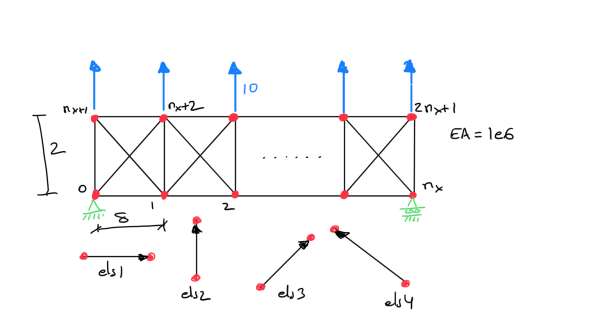
\includegraphics{celosia.png}
\caption{celosia}
\end{figure}

    \begin{tcolorbox}[breakable, size=fbox, boxrule=1pt, pad at break*=1mm,colback=cellbackground, colframe=cellborder]
\prompt{In}{incolor}{68}{\boxspacing}
\begin{Verbatim}[commandchars=\\\{\}]
\PY{n}{nx} \PY{o}{=} \PY{l+m+mi}{15}
\PY{n}{x} \PY{o}{=} \PY{n}{gennodos}\PY{p}{(}\PY{n}{xf}\PY{p}{,}\PY{n}{yf}\PY{p}{,}\PY{p}{[}\PY{l+m+mi}{0}\PY{p}{,}\PY{n}{nx}\PY{o}{*}\PY{l+m+mi}{8}\PY{p}{,}\PY{n}{nx}\PY{o}{+}\PY{l+m+mi}{1}\PY{p}{]}\PY{p}{,}\PY{p}{[}\PY{l+m+mi}{0}\PY{p}{,}\PY{l+m+mi}{2}\PY{p}{,}\PY{l+m+mi}{2}\PY{p}{]}\PY{p}{,}\PY{p}{[}\PY{p}{[}\PY{l+m+mi}{1}\PY{p}{,}\PY{l+m+mi}{1}\PY{p}{]}\PY{p}{]}\PY{p}{,}\PY{l+m+mi}{0}\PY{p}{,}\PY{l+m+mi}{2}\PY{o}{*}\PY{n}{nx}\PY{o}{+}\PY{l+m+mi}{2}\PY{p}{)}
\end{Verbatim}
\end{tcolorbox}

    \begin{tcolorbox}[breakable, size=fbox, boxrule=1pt, pad at break*=1mm,colback=cellbackground, colframe=cellborder]
\prompt{In}{incolor}{69}{\boxspacing}
\begin{Verbatim}[commandchars=\\\{\}]
\PY{n}{els1} \PY{o}{=} \PY{n}{genelem}\PY{p}{(}\PY{p}{[}\PY{p}{[}\PY{l+m+mi}{1}\PY{p}{,}\PY{l+m+mi}{1}\PY{p}{,}\PY{l+m+mi}{1}\PY{p}{]}\PY{p}{,}\PY{p}{[}\PY{l+m+mi}{1}\PY{p}{,}\PY{l+m+mi}{1}\PY{p}{,}\PY{n}{nx}\PY{p}{]}\PY{p}{]}\PY{p}{,}\PY{p}{[}\PY{l+m+mi}{0}\PY{p}{,}\PY{l+m+mi}{1}\PY{p}{]}\PY{p}{,}\PY{l+m+mi}{2}\PY{o}{*}\PY{n}{nx}\PY{p}{,}\PY{n}{x}\PY{p}{,}\PY{n}{fc}\PY{p}{(}\PY{l+m+mf}{1e6}\PY{p}{)}\PY{p}{)}
\end{Verbatim}
\end{tcolorbox}

    \begin{tcolorbox}[breakable, size=fbox, boxrule=1pt, pad at break*=1mm,colback=cellbackground, colframe=cellborder]
\prompt{In}{incolor}{70}{\boxspacing}
\begin{Verbatim}[commandchars=\\\{\}]
\PY{n}{els2} \PY{o}{=} \PY{n}{genelem}\PY{p}{(}\PY{p}{[}\PY{p}{[}\PY{l+m+mi}{1}\PY{p}{,}\PY{l+m+mi}{1}\PY{p}{,}\PY{l+m+mi}{1}\PY{p}{]}\PY{p}{]}\PY{p}{,}\PY{p}{[}\PY{l+m+mi}{0}\PY{p}{,}\PY{n}{nx}\PY{o}{+}\PY{l+m+mi}{1}\PY{p}{]}\PY{p}{,}\PY{n}{nx}\PY{o}{+}\PY{l+m+mi}{1}\PY{p}{,}\PY{n}{x}\PY{p}{,}\PY{n}{fc}\PY{p}{(}\PY{l+m+mf}{1e6}\PY{p}{)}\PY{p}{)}
\end{Verbatim}
\end{tcolorbox}

    \begin{tcolorbox}[breakable, size=fbox, boxrule=1pt, pad at break*=1mm,colback=cellbackground, colframe=cellborder]
\prompt{In}{incolor}{71}{\boxspacing}
\begin{Verbatim}[commandchars=\\\{\}]
\PY{n}{els3} \PY{o}{=} \PY{n}{genelem}\PY{p}{(}\PY{p}{[}\PY{p}{[}\PY{l+m+mi}{1}\PY{p}{,}\PY{l+m+mi}{1}\PY{p}{,}\PY{l+m+mi}{1}\PY{p}{]}\PY{p}{]}\PY{p}{,}\PY{p}{[}\PY{l+m+mi}{0}\PY{p}{,}\PY{n}{nx}\PY{o}{+}\PY{l+m+mi}{2}\PY{p}{]}\PY{p}{,}\PY{n}{nx}\PY{p}{,}\PY{n}{x}\PY{p}{,}\PY{n}{fc}\PY{p}{(}\PY{l+m+mf}{1e6}\PY{p}{)}\PY{p}{)}
\PY{n}{els4} \PY{o}{=} \PY{n}{genelem}\PY{p}{(}\PY{p}{[}\PY{p}{[}\PY{l+m+mi}{1}\PY{p}{,}\PY{l+m+mi}{1}\PY{p}{,}\PY{l+m+mi}{1}\PY{p}{]}\PY{p}{]}\PY{p}{,}\PY{p}{[}\PY{l+m+mi}{1}\PY{p}{,}\PY{n}{nx}\PY{o}{+}\PY{l+m+mi}{1}\PY{p}{]}\PY{p}{,}\PY{n}{nx}\PY{p}{,}\PY{n}{x}\PY{p}{,}\PY{n}{fc}\PY{p}{(}\PY{l+m+mf}{1e6}\PY{p}{)}\PY{p}{)}
\end{Verbatim}
\end{tcolorbox}

    \begin{tcolorbox}[breakable, size=fbox, boxrule=1pt, pad at break*=1mm,colback=cellbackground, colframe=cellborder]
\prompt{In}{incolor}{72}{\boxspacing}
\begin{Verbatim}[commandchars=\\\{\}]
\PY{n}{elementos} \PY{o}{=} \PY{n}{els1}\PY{o}{+}\PY{n}{els2}\PY{o}{+}\PY{n}{els3}\PY{o}{+}\PY{n}{els4}
\end{Verbatim}
\end{tcolorbox}

    \begin{tcolorbox}[breakable, size=fbox, boxrule=1pt, pad at break*=1mm,colback=cellbackground, colframe=cellborder]
\prompt{In}{incolor}{73}{\boxspacing}
\begin{Verbatim}[commandchars=\\\{\}]
\PY{n}{ax} \PY{o}{=} \PY{n}{plt}\PY{o}{.}\PY{n}{gca}\PY{p}{(}\PY{p}{)}
\PY{c+c1}{\PYZsh{}ax.set\PYZus{}aspect(\PYZsq{}equal\PYZsq{})}
\PY{n}{ax}\PY{o}{.}\PY{n}{set\PYZus{}aspect}\PY{p}{(}\PY{l+m+mi}{7}\PY{p}{)}
\PY{n}{f\PYZus{}dibnodos}\PY{p}{(}\PY{n}{x}\PY{p}{)}\PY{p}{;}
\PY{n}{f\PYZus{}dibelems}\PY{p}{(}\PY{n}{x}\PY{p}{,}\PY{n}{elementos}\PY{p}{)}\PY{p}{;}
\end{Verbatim}
\end{tcolorbox}

    \begin{center}
    \adjustimage{max size={0.9\linewidth}{0.9\paperheight}}{el_fin2d_files/el_fin2d_124_0.png}
    \end{center}
    { \hspace*{\fill} \\}
    
    Las condiciones de contorno son del nodo inferior izquierdo fijo y el
nodo inferior derecho con un carrito.\\
Las fuerzas son unas fuerzas concentradas en los nodos del cordón
superior.

    \begin{tcolorbox}[breakable, size=fbox, boxrule=1pt, pad at break*=1mm,colback=cellbackground, colframe=cellborder]
\prompt{In}{incolor}{74}{\boxspacing}
\begin{Verbatim}[commandchars=\\\{\}]
\PY{n}{cc} \PY{o}{=} \PY{p}{[}\PY{p}{[}\PY{l+m+mi}{0}\PY{p}{,}\PY{l+m+mi}{0}\PY{p}{]}\PY{p}{,}\PY{p}{[}\PY{l+m+mi}{0}\PY{p}{,}\PY{l+m+mi}{1}\PY{p}{]}\PY{p}{,}\PY{p}{[}\PY{n}{nx}\PY{p}{,}\PY{l+m+mi}{1}\PY{p}{]}\PY{p}{]}
\PY{n}{fuerzas} \PY{o}{=} \PY{n}{genfuerzas}\PY{p}{(}\PY{p}{[}\PY{p}{[}\PY{l+m+mi}{1}\PY{p}{,}\PY{l+m+mi}{0}\PY{p}{,}\PY{l+m+mi}{1}\PY{p}{]}\PY{p}{]}\PY{p}{,}\PY{p}{[}\PY{n}{nx}\PY{o}{+}\PY{l+m+mi}{1}\PY{p}{,}\PY{l+m+mi}{1}\PY{p}{]}\PY{p}{,}\PY{n}{nx}\PY{o}{+}\PY{l+m+mi}{1}\PY{p}{,}\PY{n}{x}\PY{p}{,}\PY{n}{fc}\PY{p}{(}\PY{l+m+mi}{10}\PY{p}{)}\PY{p}{)}
\end{Verbatim}
\end{tcolorbox}

    \begin{tcolorbox}[breakable, size=fbox, boxrule=1pt, pad at break*=1mm,colback=cellbackground, colframe=cellborder]
\prompt{In}{incolor}{75}{\boxspacing}
\begin{Verbatim}[commandchars=\\\{\}]
\PY{n}{fuerzas}
\end{Verbatim}
\end{tcolorbox}

            \begin{tcolorbox}[breakable, size=fbox, boxrule=.5pt, pad at break*=1mm, opacityfill=0]
\prompt{Out}{outcolor}{75}{\boxspacing}
\begin{Verbatim}[commandchars=\\\{\}]
[[16, 1, 10],
 [17, 1, 10],
 [18, 1, 10],
 [19, 1, 10],
 [20, 1, 10],
 [21, 1, 10],
 [22, 1, 10],
 [23, 1, 10],
 [24, 1, 10],
 [25, 1, 10],
 [26, 1, 10],
 [27, 1, 10],
 [28, 1, 10],
 [29, 1, 10],
 [30, 1, 10],
 [31, 1, 10]]
\end{Verbatim}
\end{tcolorbox}
        
    \begin{tcolorbox}[breakable, size=fbox, boxrule=1pt, pad at break*=1mm,colback=cellbackground, colframe=cellborder]
\prompt{In}{incolor}{76}{\boxspacing}
\begin{Verbatim}[commandchars=\\\{\}]
\PY{n}{u}\PY{o}{=}\PY{n}{f\PYZus{}solve}\PY{p}{(}\PY{n}{x}\PY{p}{,}\PY{n}{elementos}\PY{p}{,}\PY{n}{fuerzas}\PY{p}{,}\PY{n}{cc}\PY{p}{)}
\end{Verbatim}
\end{tcolorbox}

    Dibujo de los movimientos de la viga.

    \begin{tcolorbox}[breakable, size=fbox, boxrule=1pt, pad at break*=1mm,colback=cellbackground, colframe=cellborder]
\prompt{In}{incolor}{77}{\boxspacing}
\begin{Verbatim}[commandchars=\\\{\}]
\PY{n}{ax} \PY{o}{=} \PY{n}{plt}\PY{o}{.}\PY{n}{gca}\PY{p}{(}\PY{p}{)}
\PY{c+c1}{\PYZsh{}ax.set\PYZus{}aspect(\PYZsq{}equal\PYZsq{})}
\PY{n}{ax}\PY{o}{.}\PY{n}{set\PYZus{}aspect}\PY{p}{(}\PY{l+m+mi}{7}\PY{p}{)}
\PY{n}{f\PYZus{}dibnodos}\PY{p}{(}\PY{n}{x}\PY{o}{+}\PY{n}{u}\PY{p}{)}\PY{p}{;}
\PY{n}{f\PYZus{}dibelems}\PY{p}{(}\PY{n}{x}\PY{o}{+}\PY{n}{u}\PY{p}{,}\PY{n}{elementos}\PY{p}{)}\PY{p}{;}
\end{Verbatim}
\end{tcolorbox}

    \begin{center}
    \adjustimage{max size={0.9\linewidth}{0.9\paperheight}}{el_fin2d_files/el_fin2d_130_0.png}
    \end{center}
    { \hspace*{\fill} \\}
    
    \hypertarget{arco-parabuxf3lico-de-celosuxeda}{%
\subsection{Arco parabólico de
celosía}\label{arco-parabuxf3lico-de-celosuxeda}}

    Podemos generar el modelo con forma de arco parabólico. Basta con
utilizar las ecuaciones de la parábola.\\
En este caso para una luz de 120 metros y una flecha de 30 metros.\\
Se ha considerado que el canto de la viga se genera según la normal a la
parábola.

    \begin{tcolorbox}[breakable, size=fbox, boxrule=1pt, pad at break*=1mm,colback=cellbackground, colframe=cellborder]
\prompt{In}{incolor}{78}{\boxspacing}
\begin{Verbatim}[commandchars=\\\{\}]
\PY{n}{nx} \PY{o}{=} \PY{l+m+mi}{15}
\PY{n}{xf2} \PY{o}{=} \PY{k}{lambda} \PY{n}{u}\PY{p}{,}\PY{n}{v}\PY{p}{:} \PY{n}{u}\PY{o}{+}\PY{n}{v}\PY{o}{*}\PY{p}{(}\PY{l+m+mi}{2}\PY{o}{/}\PY{l+m+mi}{120}\PY{o}{*}\PY{n}{u}\PY{p}{)}\PY{o}{/}\PY{n}{np}\PY{o}{.}\PY{n}{sqrt}\PY{p}{(}\PY{l+m+mi}{1}\PY{o}{+}\PY{l+m+mi}{4}\PY{o}{*}\PY{p}{(}\PY{l+m+mi}{1}\PY{o}{/}\PY{l+m+mi}{120}\PY{p}{)}\PY{o}{*}\PY{p}{(}\PY{l+m+mi}{1}\PY{o}{/}\PY{l+m+mi}{120}\PY{p}{)}\PY{o}{*}\PY{n}{u}\PY{o}{*}\PY{n}{u}\PY{p}{)}
\PY{n}{yf2} \PY{o}{=} \PY{k}{lambda} \PY{n}{u}\PY{p}{,}\PY{n}{v}\PY{p}{:} \PY{o}{\PYZhy{}}\PY{l+m+mi}{1}\PY{o}{/}\PY{l+m+mi}{120}\PY{o}{*}\PY{n}{u}\PY{o}{*}\PY{n}{u}\PY{o}{+}\PY{n}{v}\PY{o}{*}\PY{l+m+mi}{1}\PY{o}{/}\PY{n}{np}\PY{o}{.}\PY{n}{sqrt}\PY{p}{(}\PY{l+m+mi}{1}\PY{o}{+}\PY{p}{(}\PY{l+m+mi}{4}\PY{o}{/}\PY{l+m+mi}{120}\PY{p}{)}\PY{o}{*}\PY{p}{(}\PY{l+m+mi}{1}\PY{o}{/}\PY{l+m+mi}{120}\PY{p}{)}\PY{o}{*}\PY{n}{u}\PY{o}{*}\PY{n}{u}\PY{p}{)}
\PY{n}{x} \PY{o}{=} \PY{n}{gennodos}\PY{p}{(}\PY{n}{xf2}\PY{p}{,}\PY{n}{yf2}\PY{p}{,}\PY{p}{[}\PY{o}{\PYZhy{}}\PY{n}{nx}\PY{o}{*}\PY{l+m+mi}{4}\PY{p}{,}\PY{n}{nx}\PY{o}{*}\PY{l+m+mi}{4}\PY{p}{,}\PY{n}{nx}\PY{o}{+}\PY{l+m+mi}{1}\PY{p}{]}\PY{p}{,}\PY{p}{[}\PY{l+m+mi}{0}\PY{p}{,}\PY{l+m+mi}{4}\PY{p}{,}\PY{l+m+mi}{2}\PY{p}{]}\PY{p}{,}\PY{p}{[}\PY{p}{[}\PY{l+m+mi}{1}\PY{p}{,}\PY{l+m+mi}{1}\PY{p}{]}\PY{p}{]}\PY{p}{,}\PY{l+m+mi}{0}\PY{p}{,}\PY{l+m+mi}{2}\PY{o}{*}\PY{n}{nx}\PY{o}{+}\PY{l+m+mi}{2}\PY{p}{)}
\end{Verbatim}
\end{tcolorbox}

    Dibujamos los nodos solamente.

    \begin{tcolorbox}[breakable, size=fbox, boxrule=1pt, pad at break*=1mm,colback=cellbackground, colframe=cellborder]
\prompt{In}{incolor}{79}{\boxspacing}
\begin{Verbatim}[commandchars=\\\{\}]
\PY{n}{ax} \PY{o}{=} \PY{n}{plt}\PY{o}{.}\PY{n}{gca}\PY{p}{(}\PY{p}{)}
\PY{n}{ax}\PY{o}{.}\PY{n}{set\PYZus{}aspect}\PY{p}{(}\PY{l+s+s1}{\PYZsq{}}\PY{l+s+s1}{equal}\PY{l+s+s1}{\PYZsq{}}\PY{p}{)}
\PY{n}{f\PYZus{}dibnodos}\PY{p}{(}\PY{n}{x}\PY{p}{)}\PY{p}{;}
\end{Verbatim}
\end{tcolorbox}

    \begin{center}
    \adjustimage{max size={0.9\linewidth}{0.9\paperheight}}{el_fin2d_files/el_fin2d_135_0.png}
    \end{center}
    { \hspace*{\fill} \\}
    
    Los elementos son exactamente los mismos que en el caso anterior.

    \begin{tcolorbox}[breakable, size=fbox, boxrule=1pt, pad at break*=1mm,colback=cellbackground, colframe=cellborder]
\prompt{In}{incolor}{80}{\boxspacing}
\begin{Verbatim}[commandchars=\\\{\}]
\PY{n}{els1} \PY{o}{=} \PY{n}{genelem}\PY{p}{(}\PY{p}{[}\PY{p}{[}\PY{l+m+mi}{1}\PY{p}{,}\PY{l+m+mi}{1}\PY{p}{,}\PY{l+m+mi}{1}\PY{p}{]}\PY{p}{,}\PY{p}{[}\PY{l+m+mi}{1}\PY{p}{,}\PY{l+m+mi}{1}\PY{p}{,}\PY{n}{nx}\PY{p}{]}\PY{p}{]}\PY{p}{,}\PY{p}{[}\PY{l+m+mi}{0}\PY{p}{,}\PY{l+m+mi}{1}\PY{p}{]}\PY{p}{,}\PY{l+m+mi}{2}\PY{o}{*}\PY{n}{nx}\PY{p}{,}\PY{n}{x}\PY{p}{,}\PY{n}{fc}\PY{p}{(}\PY{l+m+mf}{1e6}\PY{p}{)}\PY{p}{)}
\end{Verbatim}
\end{tcolorbox}

    \begin{tcolorbox}[breakable, size=fbox, boxrule=1pt, pad at break*=1mm,colback=cellbackground, colframe=cellborder]
\prompt{In}{incolor}{81}{\boxspacing}
\begin{Verbatim}[commandchars=\\\{\}]
\PY{n}{els2} \PY{o}{=} \PY{n}{genelem}\PY{p}{(}\PY{p}{[}\PY{p}{[}\PY{l+m+mi}{1}\PY{p}{,}\PY{l+m+mi}{1}\PY{p}{,}\PY{l+m+mi}{1}\PY{p}{]}\PY{p}{]}\PY{p}{,}\PY{p}{[}\PY{l+m+mi}{0}\PY{p}{,}\PY{n}{nx}\PY{o}{+}\PY{l+m+mi}{1}\PY{p}{]}\PY{p}{,}\PY{n}{nx}\PY{o}{+}\PY{l+m+mi}{1}\PY{p}{,}\PY{n}{x}\PY{p}{,}\PY{n}{fc}\PY{p}{(}\PY{l+m+mf}{1e6}\PY{p}{)}\PY{p}{)}
\end{Verbatim}
\end{tcolorbox}

    \begin{tcolorbox}[breakable, size=fbox, boxrule=1pt, pad at break*=1mm,colback=cellbackground, colframe=cellborder]
\prompt{In}{incolor}{82}{\boxspacing}
\begin{Verbatim}[commandchars=\\\{\}]
\PY{n}{els3} \PY{o}{=} \PY{n}{genelem}\PY{p}{(}\PY{p}{[}\PY{p}{[}\PY{l+m+mi}{1}\PY{p}{,}\PY{l+m+mi}{1}\PY{p}{,}\PY{l+m+mi}{1}\PY{p}{]}\PY{p}{]}\PY{p}{,}\PY{p}{[}\PY{l+m+mi}{0}\PY{p}{,}\PY{n}{nx}\PY{o}{+}\PY{l+m+mi}{2}\PY{p}{]}\PY{p}{,}\PY{n}{nx}\PY{p}{,}\PY{n}{x}\PY{p}{,}\PY{n}{fc}\PY{p}{(}\PY{l+m+mf}{1e6}\PY{p}{)}\PY{p}{)}
\PY{n}{els4} \PY{o}{=} \PY{n}{genelem}\PY{p}{(}\PY{p}{[}\PY{p}{[}\PY{l+m+mi}{1}\PY{p}{,}\PY{l+m+mi}{1}\PY{p}{,}\PY{l+m+mi}{1}\PY{p}{]}\PY{p}{]}\PY{p}{,}\PY{p}{[}\PY{l+m+mi}{1}\PY{p}{,}\PY{n}{nx}\PY{o}{+}\PY{l+m+mi}{1}\PY{p}{]}\PY{p}{,}\PY{n}{nx}\PY{p}{,}\PY{n}{x}\PY{p}{,}\PY{n}{fc}\PY{p}{(}\PY{l+m+mf}{1e6}\PY{p}{)}\PY{p}{)}
\end{Verbatim}
\end{tcolorbox}

    \begin{tcolorbox}[breakable, size=fbox, boxrule=1pt, pad at break*=1mm,colback=cellbackground, colframe=cellborder]
\prompt{In}{incolor}{83}{\boxspacing}
\begin{Verbatim}[commandchars=\\\{\}]
\PY{n}{elementos} \PY{o}{=} \PY{n}{els1}\PY{o}{+}\PY{n}{els2}\PY{o}{+}\PY{n}{els3}\PY{o}{+}\PY{n}{els4}
\end{Verbatim}
\end{tcolorbox}

    \begin{tcolorbox}[breakable, size=fbox, boxrule=1pt, pad at break*=1mm,colback=cellbackground, colframe=cellborder]
\prompt{In}{incolor}{84}{\boxspacing}
\begin{Verbatim}[commandchars=\\\{\}]
\PY{n}{ax} \PY{o}{=} \PY{n}{plt}\PY{o}{.}\PY{n}{gca}\PY{p}{(}\PY{p}{)}
\PY{n}{ax}\PY{o}{.}\PY{n}{set\PYZus{}aspect}\PY{p}{(}\PY{l+s+s1}{\PYZsq{}}\PY{l+s+s1}{equal}\PY{l+s+s1}{\PYZsq{}}\PY{p}{)}
\PY{n}{f\PYZus{}dibnodos}\PY{p}{(}\PY{n}{x}\PY{p}{)}\PY{p}{;}
\PY{n}{f\PYZus{}dibelems}\PY{p}{(}\PY{n}{x}\PY{p}{,}\PY{n}{elementos}\PY{p}{)}\PY{p}{;}
\end{Verbatim}
\end{tcolorbox}

    \begin{center}
    \adjustimage{max size={0.9\linewidth}{0.9\paperheight}}{el_fin2d_files/el_fin2d_141_0.png}
    \end{center}
    { \hspace*{\fill} \\}
    
    \begin{tcolorbox}[breakable, size=fbox, boxrule=1pt, pad at break*=1mm,colback=cellbackground, colframe=cellborder]
\prompt{In}{incolor}{85}{\boxspacing}
\begin{Verbatim}[commandchars=\\\{\}]
\PY{n}{cc} \PY{o}{=} \PY{p}{[}\PY{p}{[}\PY{l+m+mi}{0}\PY{p}{,}\PY{l+m+mi}{0}\PY{p}{]}\PY{p}{,}\PY{p}{[}\PY{l+m+mi}{0}\PY{p}{,}\PY{l+m+mi}{1}\PY{p}{]}\PY{p}{,}\PY{p}{[}\PY{n}{nx}\PY{p}{,}\PY{l+m+mi}{1}\PY{p}{]}\PY{p}{]}
\PY{n}{fuerzas} \PY{o}{=} \PY{n}{genfuerzas}\PY{p}{(}\PY{p}{[}\PY{p}{[}\PY{l+m+mi}{1}\PY{p}{,}\PY{l+m+mi}{0}\PY{p}{,}\PY{l+m+mi}{1}\PY{p}{]}\PY{p}{]}\PY{p}{,}\PY{p}{[}\PY{n}{nx}\PY{o}{+}\PY{l+m+mi}{1}\PY{p}{,}\PY{l+m+mi}{1}\PY{p}{]}\PY{p}{,}\PY{n}{nx}\PY{o}{+}\PY{l+m+mi}{1}\PY{p}{,}\PY{n}{x}\PY{p}{,}\PY{n}{fc}\PY{p}{(}\PY{o}{\PYZhy{}}\PY{l+m+mi}{10}\PY{p}{)}\PY{p}{)}
\end{Verbatim}
\end{tcolorbox}

    \begin{tcolorbox}[breakable, size=fbox, boxrule=1pt, pad at break*=1mm,colback=cellbackground, colframe=cellborder]
\prompt{In}{incolor}{86}{\boxspacing}
\begin{Verbatim}[commandchars=\\\{\}]
\PY{n}{u}\PY{o}{=}\PY{n}{f\PYZus{}solve}\PY{p}{(}\PY{n}{x}\PY{p}{,}\PY{n}{elementos}\PY{p}{,}\PY{n}{fuerzas}\PY{p}{,}\PY{n}{cc}\PY{p}{)}
\end{Verbatim}
\end{tcolorbox}

    Dibujamos los nodos sin deformar y los elementos según la deformada
amplificada $10$ veces.

    \begin{tcolorbox}[breakable, size=fbox, boxrule=1pt, pad at break*=1mm,colback=cellbackground, colframe=cellborder]
\prompt{In}{incolor}{87}{\boxspacing}
\begin{Verbatim}[commandchars=\\\{\}]
\PY{n}{ax} \PY{o}{=} \PY{n}{plt}\PY{o}{.}\PY{n}{gca}\PY{p}{(}\PY{p}{)}
\PY{n}{ax}\PY{o}{.}\PY{n}{set\PYZus{}aspect}\PY{p}{(}\PY{l+s+s1}{\PYZsq{}}\PY{l+s+s1}{equal}\PY{l+s+s1}{\PYZsq{}}\PY{p}{)}
\PY{n}{f\PYZus{}dibnodos}\PY{p}{(}\PY{n}{x}\PY{p}{)}\PY{p}{;}
\PY{n}{f\PYZus{}dibelems}\PY{p}{(}\PY{n}{x}\PY{o}{+}\PY{n}{u}\PY{o}{*}\PY{l+m+mi}{10}\PY{p}{,}\PY{n}{elementos}\PY{p}{)}\PY{p}{;}
\end{Verbatim}
\end{tcolorbox}

    \begin{center}
    \adjustimage{max size={0.9\linewidth}{0.9\paperheight}}{el_fin2d_files/el_fin2d_145_0.png}
    \end{center}
    { \hspace*{\fill} \\}
    
    Aparte de los movimientos y de los axiles que ya hemos visto como se
obtienen también podemos obtener las reacciones, que serán las fuerzas
asociadas a las restricciones. En este caso, por ejemplo,las reacciones
verticales están asociadas a los nodos u{[}0{]} y u{[}nx{]}.\\
Como el apoyo derecho es un carrito y no hay fuerzas horizontales las
únicas reacciones son las verticales que se pueden obtener multiplicando
los movimientos de los nodos coaccionados por la constante de
penalización $kpen$\\
Las fuerzas aplicadas son unas fuerzas concentradas en los nodos
superiores de valor $-10$ que hacen un total de $-160$.

    \begin{tcolorbox}[breakable, size=fbox, boxrule=1pt, pad at break*=1mm,colback=cellbackground, colframe=cellborder]
\prompt{In}{incolor}{88}{\boxspacing}
\begin{Verbatim}[commandchars=\\\{\}]
\PY{n}{u}\PY{p}{[}\PY{l+m+mi}{0}\PY{p}{]}
\end{Verbatim}
\end{tcolorbox}

            \begin{tcolorbox}[breakable, size=fbox, boxrule=.5pt, pad at break*=1mm, opacityfill=0]
\prompt{Out}{outcolor}{88}{\boxspacing}
\begin{Verbatim}[commandchars=\\\{\}]
array([ 5.85482703e-32, -8.00000000e-19])
\end{Verbatim}
\end{tcolorbox}
        
    \begin{tcolorbox}[breakable, size=fbox, boxrule=1pt, pad at break*=1mm,colback=cellbackground, colframe=cellborder]
\prompt{In}{incolor}{89}{\boxspacing}
\begin{Verbatim}[commandchars=\\\{\}]
\PY{n}{u}\PY{p}{[}\PY{n}{nx}\PY{p}{]}
\end{Verbatim}
\end{tcolorbox}

            \begin{tcolorbox}[breakable, size=fbox, boxrule=.5pt, pad at break*=1mm, opacityfill=0]
\prompt{Out}{outcolor}{89}{\boxspacing}
\begin{Verbatim}[commandchars=\\\{\}]
array([ 5.93152636e-01, -8.00000000e-19])
\end{Verbatim}
\end{tcolorbox}
        
    \begin{tcolorbox}[breakable, size=fbox, boxrule=1pt, pad at break*=1mm,colback=cellbackground, colframe=cellborder]
\prompt{In}{incolor}{90}{\boxspacing}
\begin{Verbatim}[commandchars=\\\{\}]
\PY{n}{u}\PY{p}{[}\PY{l+m+mi}{0}\PY{p}{]}\PY{p}{[}\PY{l+m+mi}{1}\PY{p}{]}\PY{o}{*}\PY{n}{kpen}
\end{Verbatim}
\end{tcolorbox}

            \begin{tcolorbox}[breakable, size=fbox, boxrule=.5pt, pad at break*=1mm, opacityfill=0]
\prompt{Out}{outcolor}{90}{\boxspacing}
\begin{Verbatim}[commandchars=\\\{\}]
-79.99999999996999
\end{Verbatim}
\end{tcolorbox}
        
    \begin{tcolorbox}[breakable, size=fbox, boxrule=1pt, pad at break*=1mm,colback=cellbackground, colframe=cellborder]
\prompt{In}{incolor}{91}{\boxspacing}
\begin{Verbatim}[commandchars=\\\{\}]
\PY{n}{u}\PY{p}{[}\PY{n}{nx}\PY{p}{]}\PY{p}{[}\PY{l+m+mi}{1}\PY{p}{]}\PY{o}{*}\PY{n}{kpen}
\end{Verbatim}
\end{tcolorbox}

            \begin{tcolorbox}[breakable, size=fbox, boxrule=.5pt, pad at break*=1mm, opacityfill=0]
\prompt{Out}{outcolor}{91}{\boxspacing}
\begin{Verbatim}[commandchars=\\\{\}]
-79.99999999996753
\end{Verbatim}
\end{tcolorbox}
        
    \begin{tcolorbox}[breakable, size=fbox, boxrule=1pt, pad at break*=1mm,colback=cellbackground, colframe=cellborder]
\prompt{In}{incolor}{ }{\boxspacing}
\begin{Verbatim}[commandchars=\\\{\}]

\end{Verbatim}
\end{tcolorbox}


    % Add a bibliography block to the postdoc
    
    
    
\end{document}
